\section{Electromagnetically Induced Transparency}
Electromagnetically Induced Tranparency is a well known phenomenon in atomic physics but its all-optical analogue has generated a lot of interest in this beautiful natural phenomenon. Basically, EIT is a transparency window in transmission and absorption spectrum. This transparency window is the result of fano interference amoung different transition pathways. There is another similar concept which is known as Autler-Townes Splitting ATS, which also shows a transparency window but it is the result of strong field-driven interactions which causes the energy levels to split.

EIT also enables us to hold control over the optical response of the medium. Basically, EIT is the result of having a strong connection between the light and the matter. Amplitudes of different pathways interfere due to quantum interference effects. These can be used in applications such as all-optical switching, slow light, optical sensing, light storage and quantum information processing.

In photonics, EIT is said to be observed in plasmonic structures, photonic crystals, whispering gallery mode micro cavities and coupled ring micro resonators. These devices can be summed up under one name, photonic devices and by seeing such effects we can say that we can get control of how information and energy travel through our device.

\subsection{EIT in Atoms}
For EIT to happen classically, one may assume that all the oscillating atoms in the medium have came to a hault just to neutralize the incoming field effect and thus these electrons does not contribute in the dielectric of the material. But atoms are small and must be treated quantum mechanically, in which we deal with probability amplitudes and expected value of electron's position. For EIT to occur, we must have a three-level atomic system which we will discuss below.
\subsection{Three level Atoms}
In a three level system, what really happens quantum mechanically, without disrupting the escence of classical phenomenons, The probability amplitudes of level $\ket{3}$ is driven by two terms in the system. One is being the probability amplitude of the ground state $\ket{1}$ and the other is the oppositely phased and is the probability amplitude of the state $\ket{2}$. These both driving forces are opposite in signs but equal in magnitudes and have a frequecy $\omega_{p}$ and are so balanced that probabilty amplitude of state $\ket{3}$ and the expected value of the amplitude of the sinosoidal motion at every frequency that has been applied is zero. 

\begin{figure}[h]
\centering
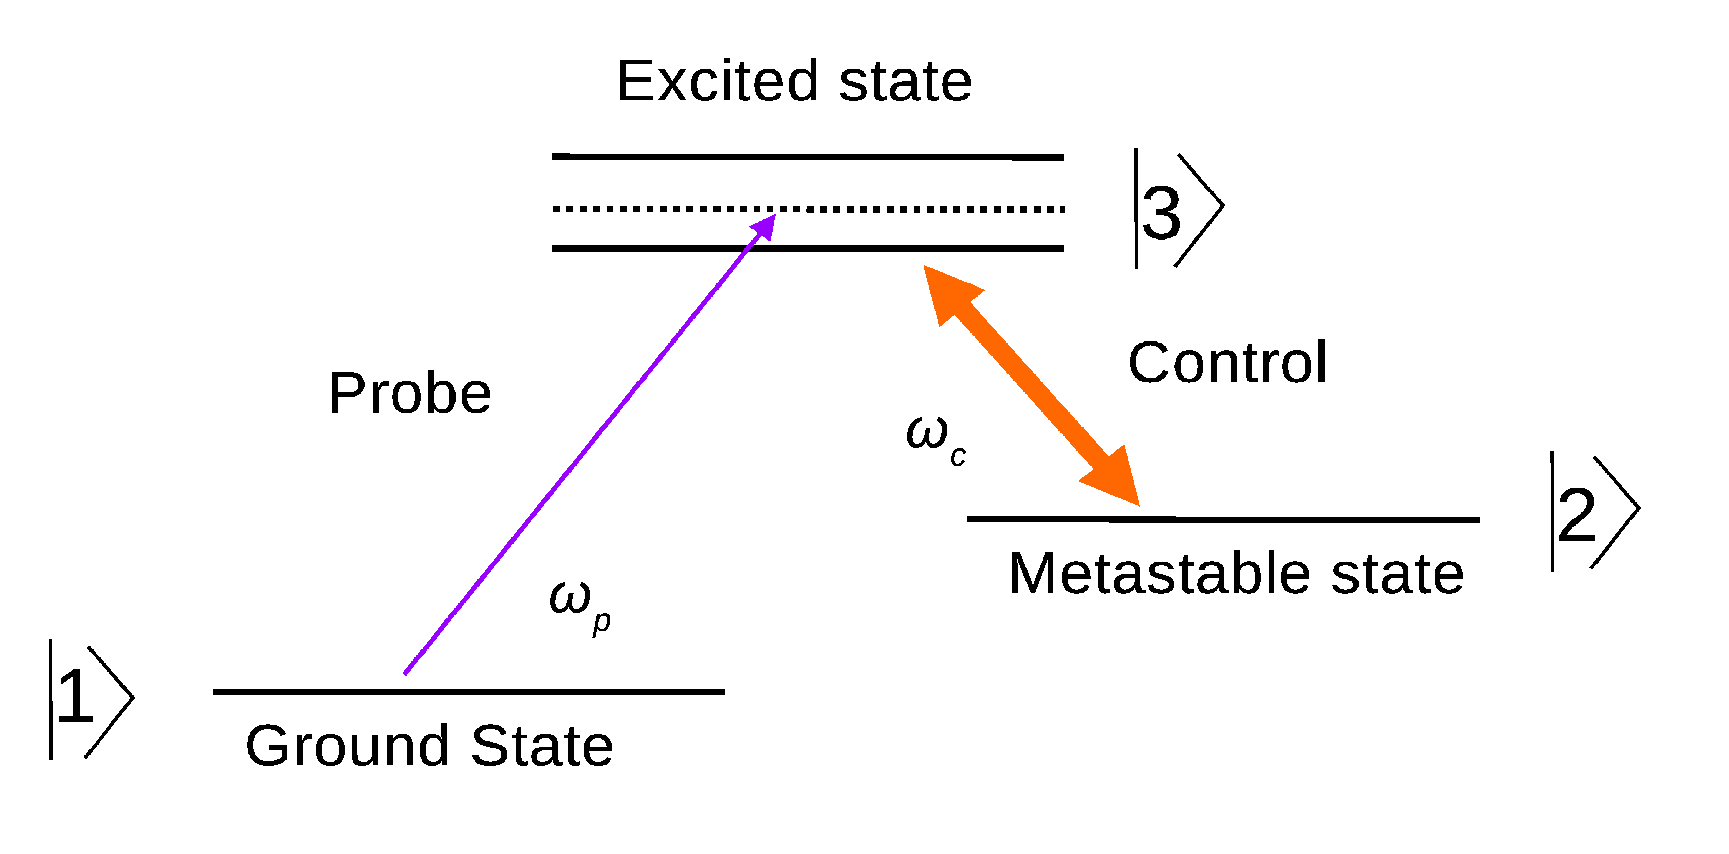
\includegraphics[scale=0.5]{EIT_3_level.eps}
\caption{A three-level system where level 3 splits due to the much stronger field of control laser.}
\end{figure}

One may ask how that opposite phase for transition from the coherent states $\ket{1} \to \ket{2}$ along with the applied field $\omega_{c}$, makes absolute cancellation? Because, we use the laser pulses that generates fast enough laser photons that the phase of transitions is maintain and is the correct phase for cancellation. 


\section{Coupled Resonator Induced Transparency (CRIT)}
We can observe EIT in coupled resonator systems as well as in other optical systems like whispering gallery resonators but the scope of this thesis is limited to ring resonators systems only. This kind of geometry (that we discussed in section 2.4) has been promising since a long time in the field of photonics. EIT can be observed in this system by mostly the explaination of classical wave travel and quantum fluctuations. The traveling photon is coupled inside the first ring through evanescent wave and travels inside the ring and acquires a phase shift equal to the round trip inside the optical cavity. When the light source and the phase shifted intracavity field matches so as that the constructive interference is amplified i-e their phases matches perfectly, then at those frequency there is a transparency window in the absorption spectrum i.e a narrow dip, or we see a sharp peak in the transmission spectrum. [2] 

\begin{figure}[h]
\centering
\includegraphics[scale=1]{coupled_ring_EIT1.png}
\caption{Electromagnetically Induced Transparency observed in a 2 ring resonator system.}
\end{figure}

\subsubsection{Transmittance}
Figure 3.2 displays the plot of transmitted intensity vs frequency detuning in a coupled resonator system as shown in fig. 2.16. The parameters used here are couplings $r_{1} = 0.9$ and $r_{2} = 0.999$ and attenuations $a_{1} = 0.88$ and $a_{2} = 0.9999$ for ring 1 and 2 respectively. Reproduced from the original work on \textit{Coupled resonator induced transparency} [2] from 2004.


\subsubsection{Effective Phase}

Now let us look at the phase response of such coupled resonator system. Figure 3.3 shows effective phase of the system in red and Figure 3.4 shows the coupling phase which is the phase between the two coupled rings, in yellow. 

\begin{figure}[h]
\includegraphics[scale=0.75]{coupled_ring_EIT1_phase.png}
\includegraphics[scale=0.75]{coupled_ring_EIT1_coupling.png}
\caption{Effective phase of the system in red and coupling phase shown in yellow vs frequency detuning.}
\end{figure}

\subsubsection{Effective Phase derivative}
Figure 3.4 shows the derivative of the phase of the system which gives us great information about the group index and group velocity of the system. 

This value is directly related to the group index of the system. From the graph, we can see that there are negative values for off resonances and positive values on resonances. Which tells us that we have superluminal light off resonance and subluminal on resonance. 
\begin{figure}[h]
\centering
\includegraphics[scale=1]{coupled_ring_EIT1_deri.png}
\caption{Derivative of the phase of the system vs frequency detuning.}
\end{figure}

\newpage
\subsection{CRIT with gain}
As before, now we are going to observe what changes does the system has when we introduce gain in it. This can be introduced by pumping some monochromatic light source or a laser, in either one of the rings which will drastically incompensate the losses inside the resonator and will increase the overall output transmission of the system even above the incident light source. 
\subsection{Results}
We observe EIT in a coupled two resonator system, the transmission and effective phase of the system is shown displaying normal dispersion meaning slow light in the system.

\begin{figure}[h]
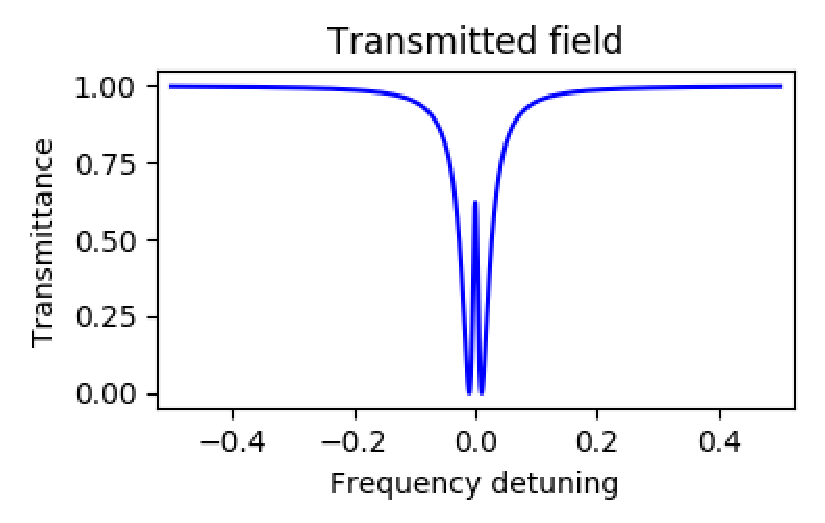
\includegraphics[scale=0.5]{EIT_1.eps}
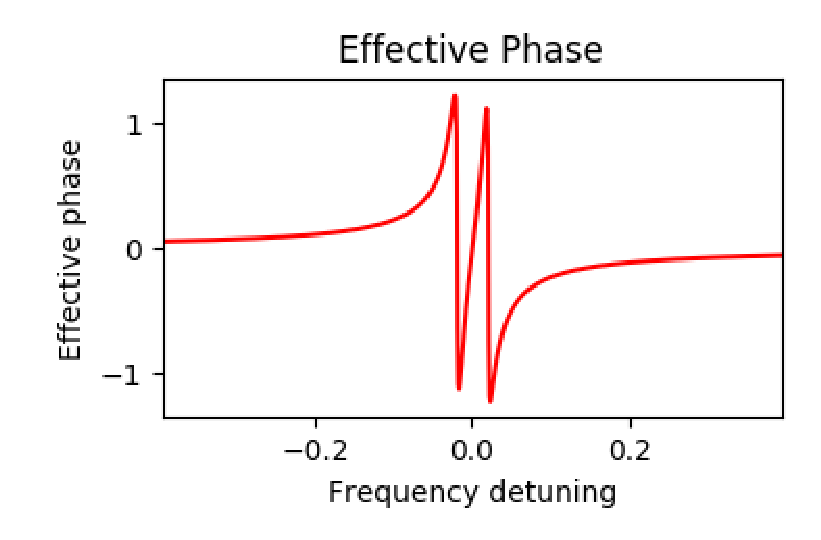
\includegraphics[scale=0.5]{EIT_phase.eps}
\caption{Coupled Resonator Induced Transparency with its effective phase in a passive resonator system.}
\end{figure}

\subsubsection{Introducing gain in resonator 2}
Now we will activate gain in the resonator 2, which has high Quality-factor (shown in red in fig. 3.6). The transmission peak of the EIT starts to rise up gradually as $g$ , the gain coefficient, is increased. The peak rises towards 1 mark up till $g \to \alpha$, where alpha is the attenuation constant. 

\begin{figure}[h]
\centering
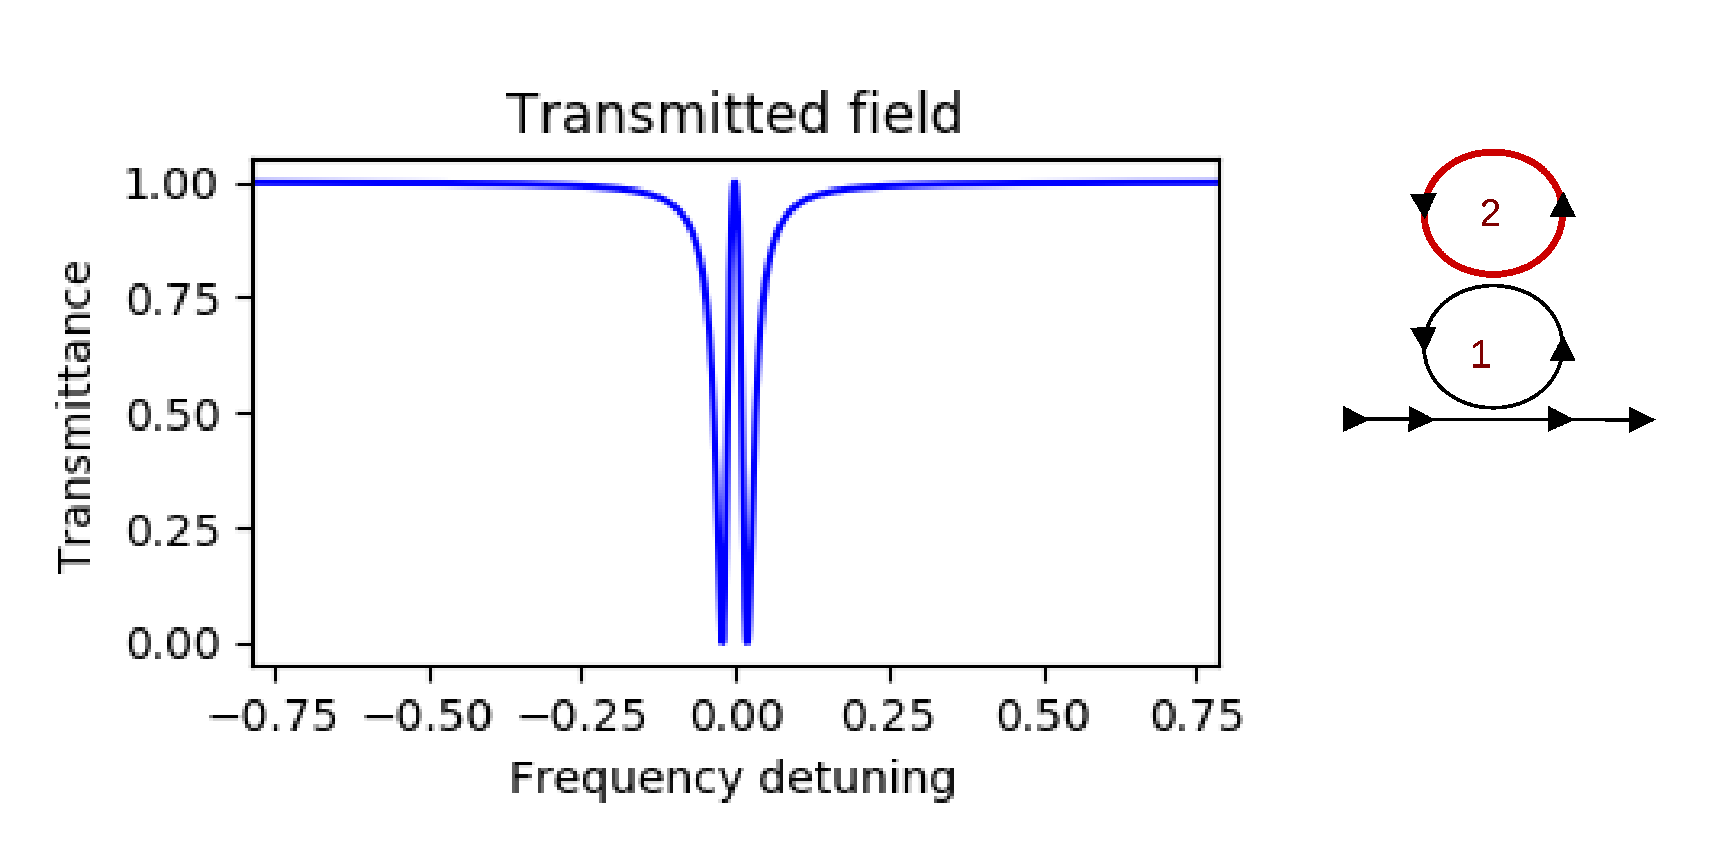
\includegraphics[scale=0.5]{EIT_gain2.eps}
\caption{Coupled Resonator Induced Transparency with in an active resonator system.}
\end{figure}

When $g = \alpha$ , the peak of the transmission touches the 1 mark on the graph meaning now all of the incident intensity is being detected on the other side i.e it has become completely transparent. This means that we have now compensated for all the losses inside the system which can be intrinsic, coupling or bending losses. When this happens, we see an abrupt change in thae effective phase of the system. This system now gives us anamolous dispersion on resonance meaning we get fast light in EIT. 

To get a brief idea of what is really happenning, I have also calculated the group index of the system. In this case, we receive negative values for the group index $n_{g}$ on resonance. Fig. 3.8 displays the group index for this particular case.


\begin{figure}[t]
\centering
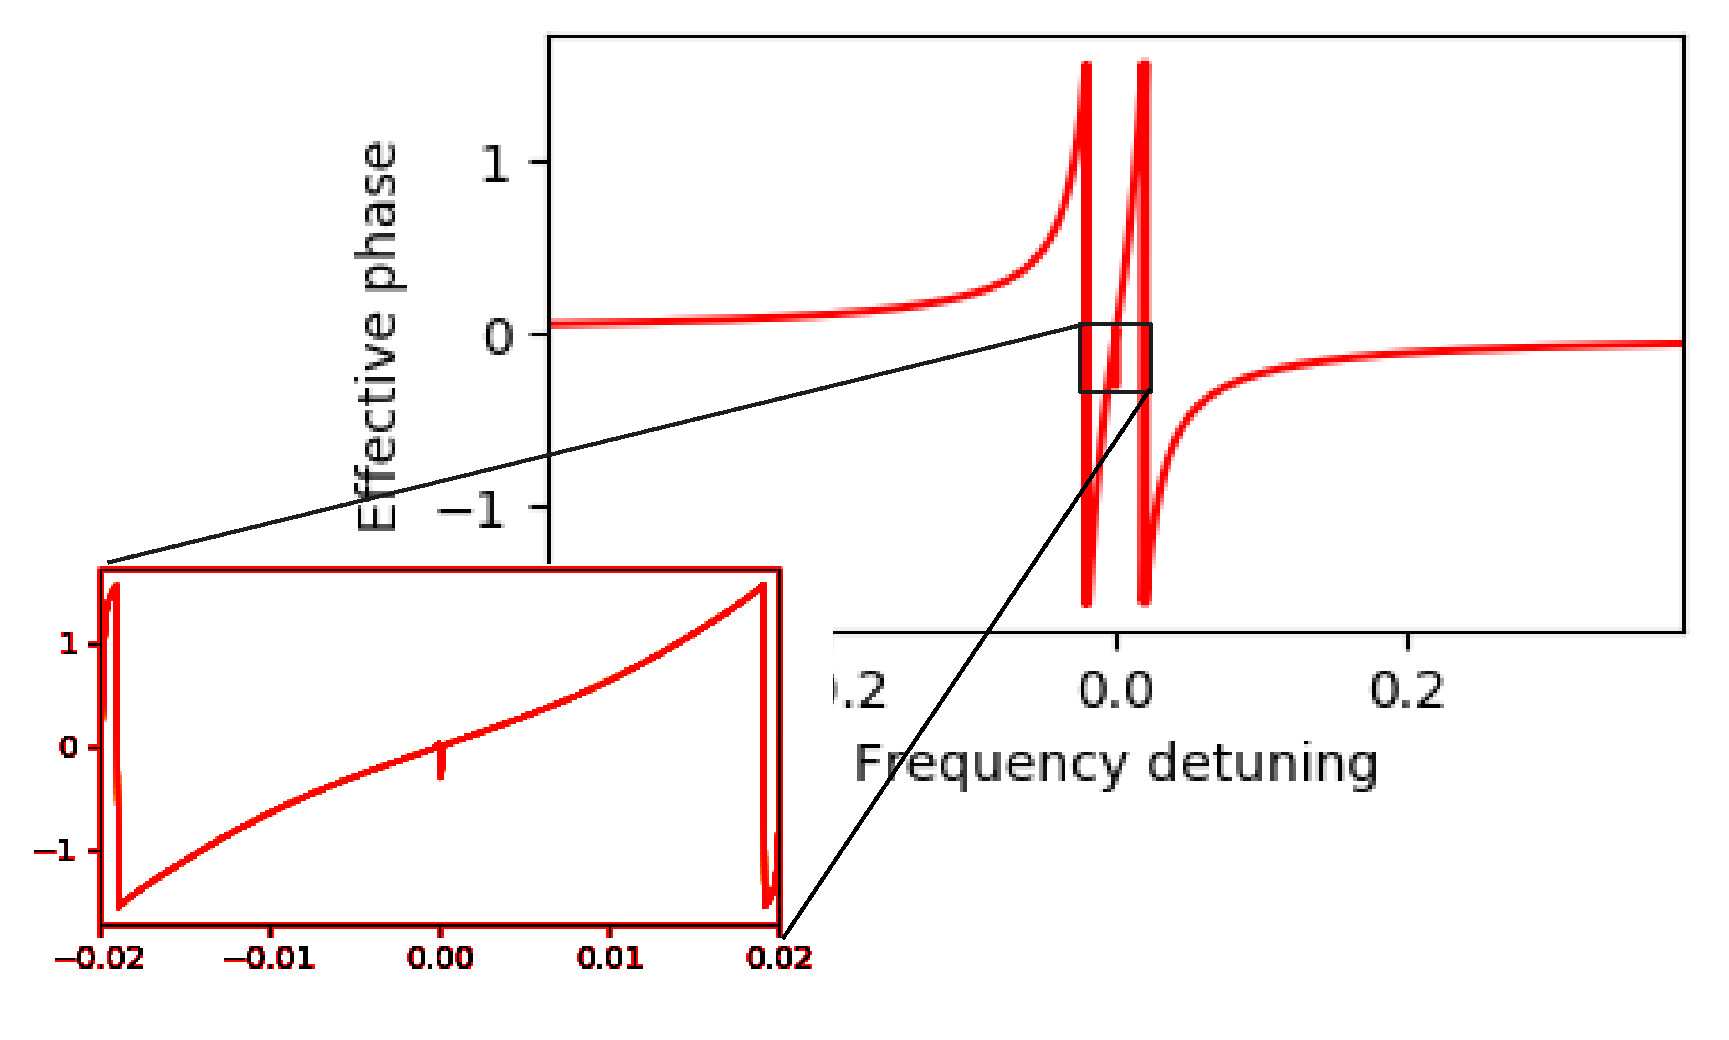
\includegraphics[scale=0.35]{EIT_gain2_phase.eps}
\caption{Effective phase of Coupled Resonator Induced Transparency  in an active resonator system.}
\end{figure}

 	
\begin{figure}[h]
\centering
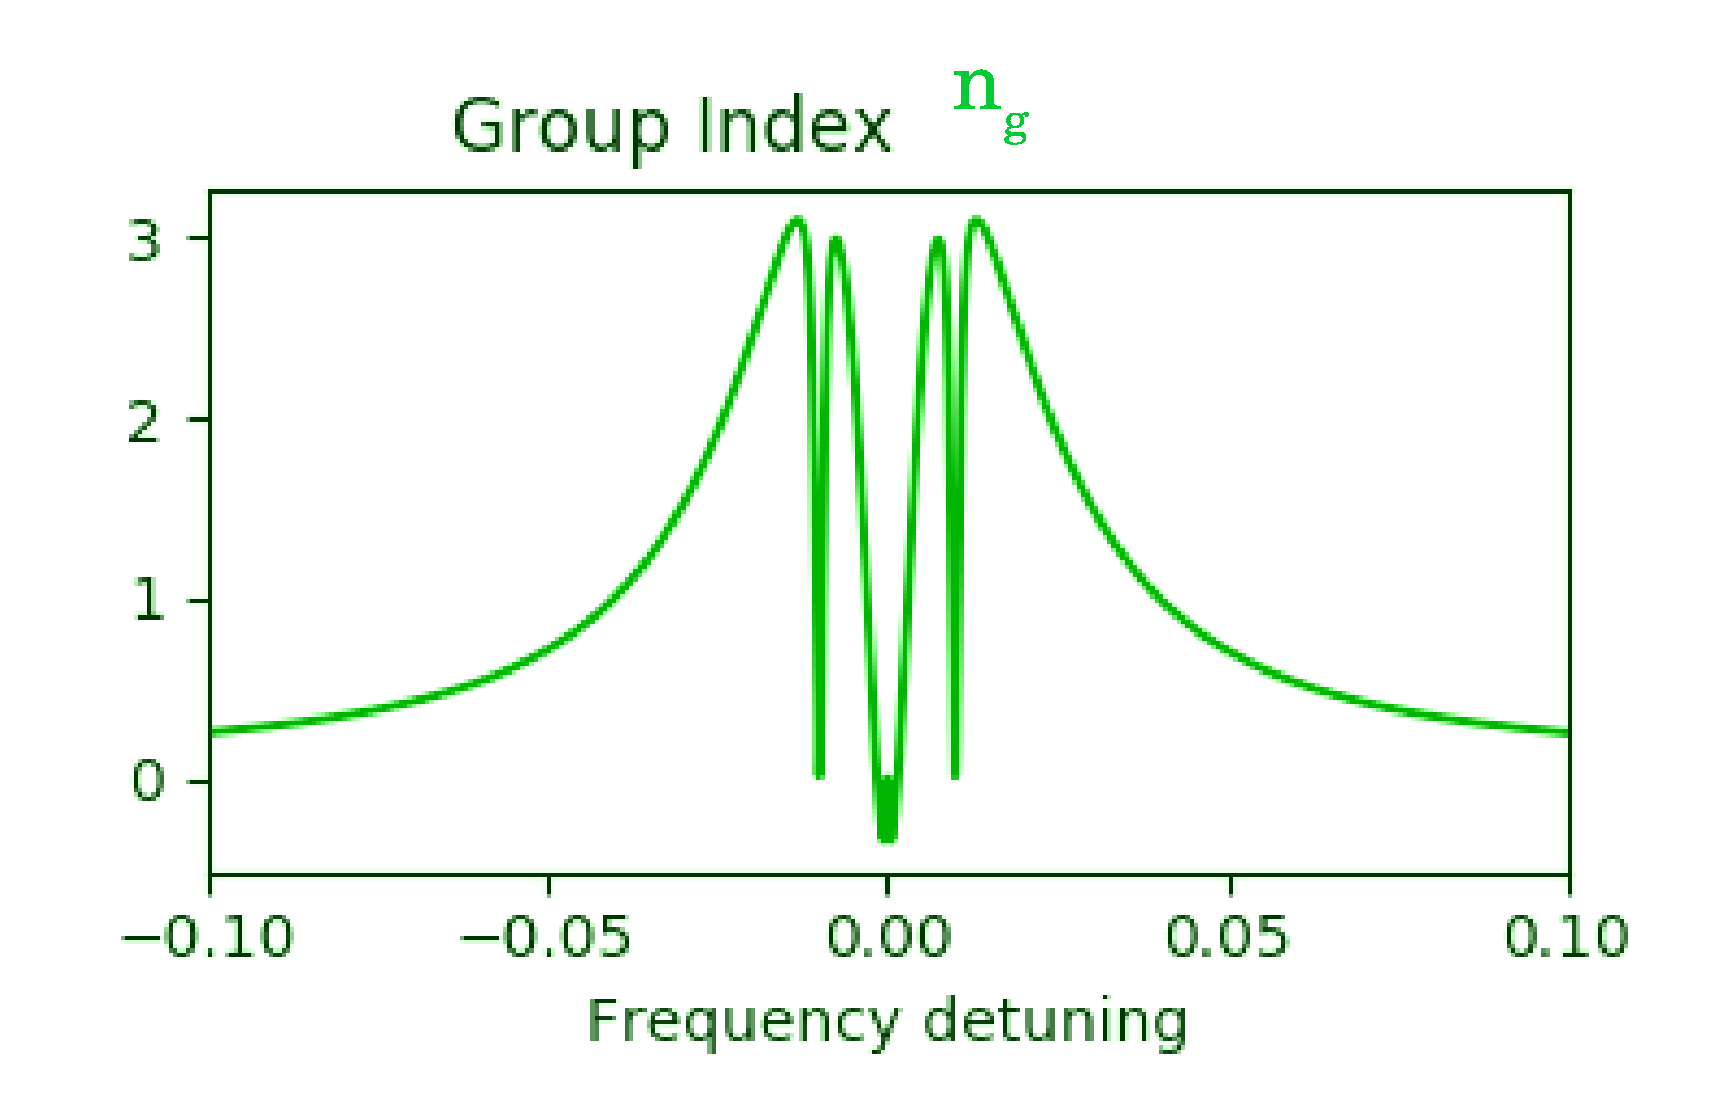
\includegraphics[scale=0.35]{EIT_gain2_ng.eps}
\caption{Group index of Coupled Resonator Induced Transparency  in an active resonator system showing negative on resonant frequencies.}
\end{figure}
\newpage

\subsubsection{Introducing gain in resonator 1}
Now we will activate gain in resonator 1 (shown in red), which has lower Quality-factor in comparison to the resonator 2. The spectrum of the EIT starts to rise up and displays a hanging EIT closer to the 1 mark on the graph. (Figure 3.9)

\begin{figure}[h]
\centering
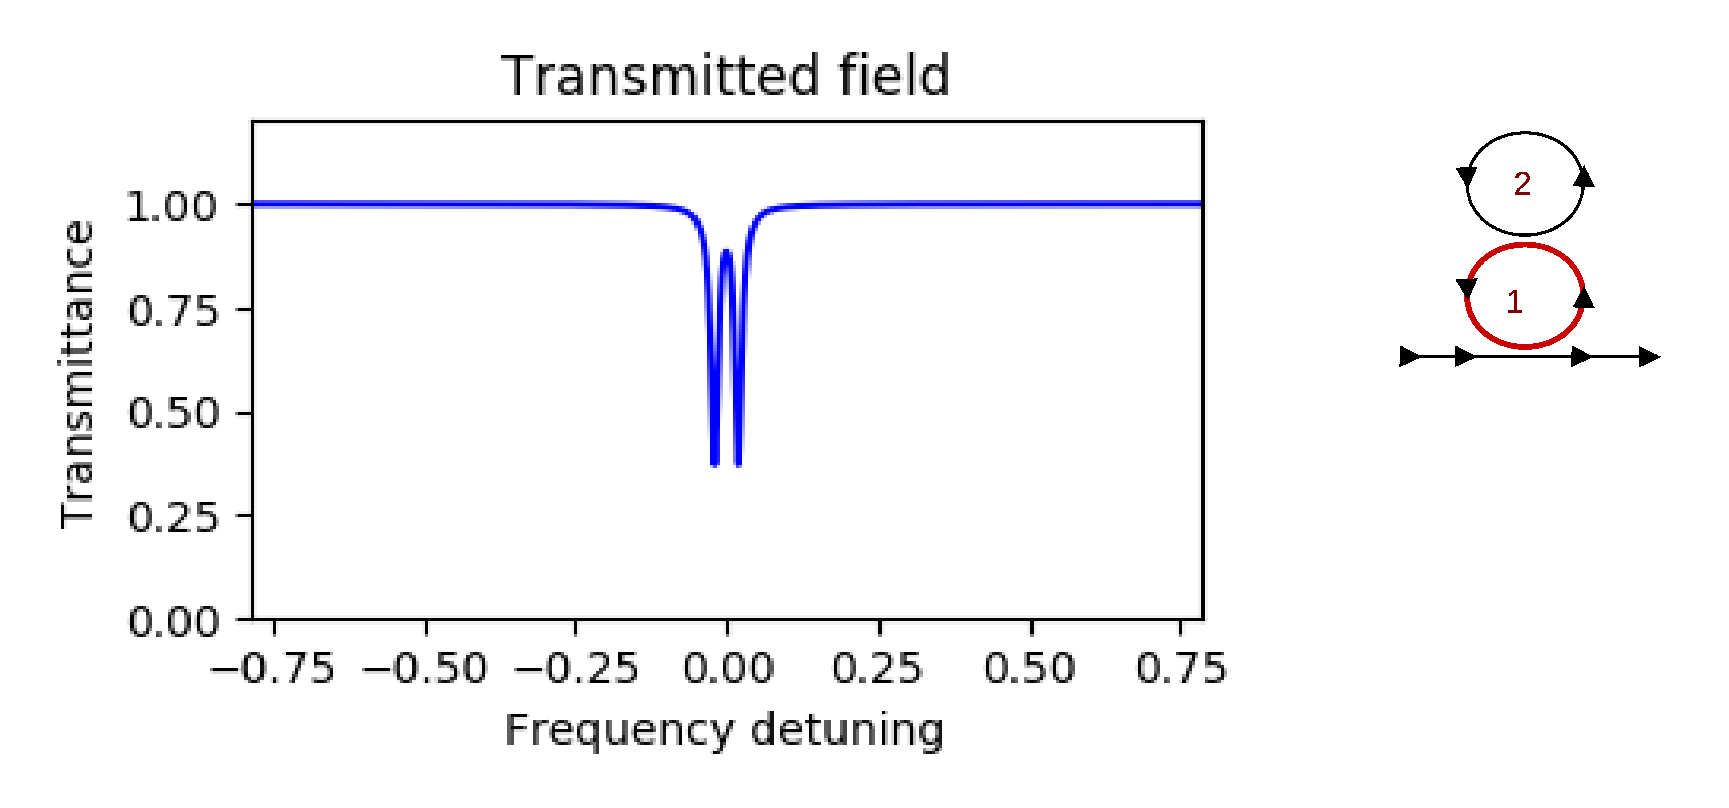
\includegraphics[scale=0.35]{EIT_gain1.eps}
\caption{CRIT of the 2 resonator system with gain activated in resonantor 1.}
\end{figure}

The effective phase of the system remains the same as of a passive resonator, displayin normal dispersion meaning slow light. As we can also see from the group index. The index value on resonance calculated to be about $\approx 76.2$ which displays a very less reduction in the speed of light. 

\begin{figure}[h]
\includegraphics[scale=0.5]{EIT_gain1_phase.png}
\includegraphics[scale=0.5]{EIT_gain1_ng.png}
\caption{Effective phase shows normal dispersion (in red) and group index $n_{g}$ shown in green.}
\end{figure}


\subsubsection{Introducing gain in both resonators}
Now we will activate gain in both of the resonators simultaneously such that the ratio of the gain coefficients, $g_{1}$ and $g_{2}$, are the same. 
We observe that the peak of the EIT as well as the whole transmission starts to rise up towards the 1 mark as $g \to \alpha$ Fig. 3.11. The EIT transmission window also narrows down gradually.

\begin{figure}[h]
\centering
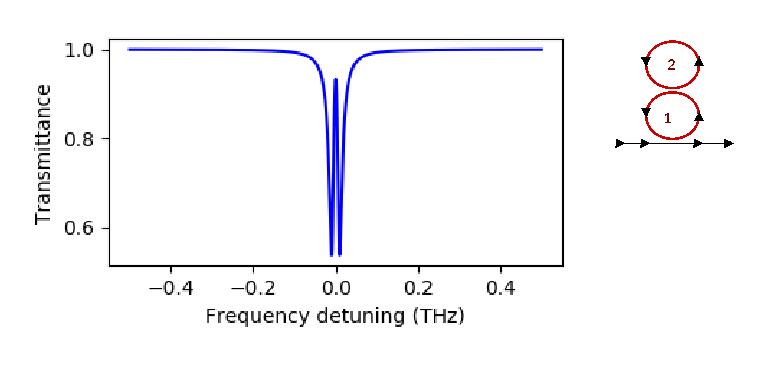
\includegraphics[scale=0.70]{EIT_gain12.eps}
\caption{Transmission graph of two resonator system with gain activated in both (shown in red).}
\end{figure}

The effective phase of the system shows a rather distinct curves which are basically due to the artifacts in the system of computation errors. The on resonance information tells us that we have normal dispersion and positive group index about $\approx 766.5$ Fig. 3.12. 

\begin{figure}[h]
\centering
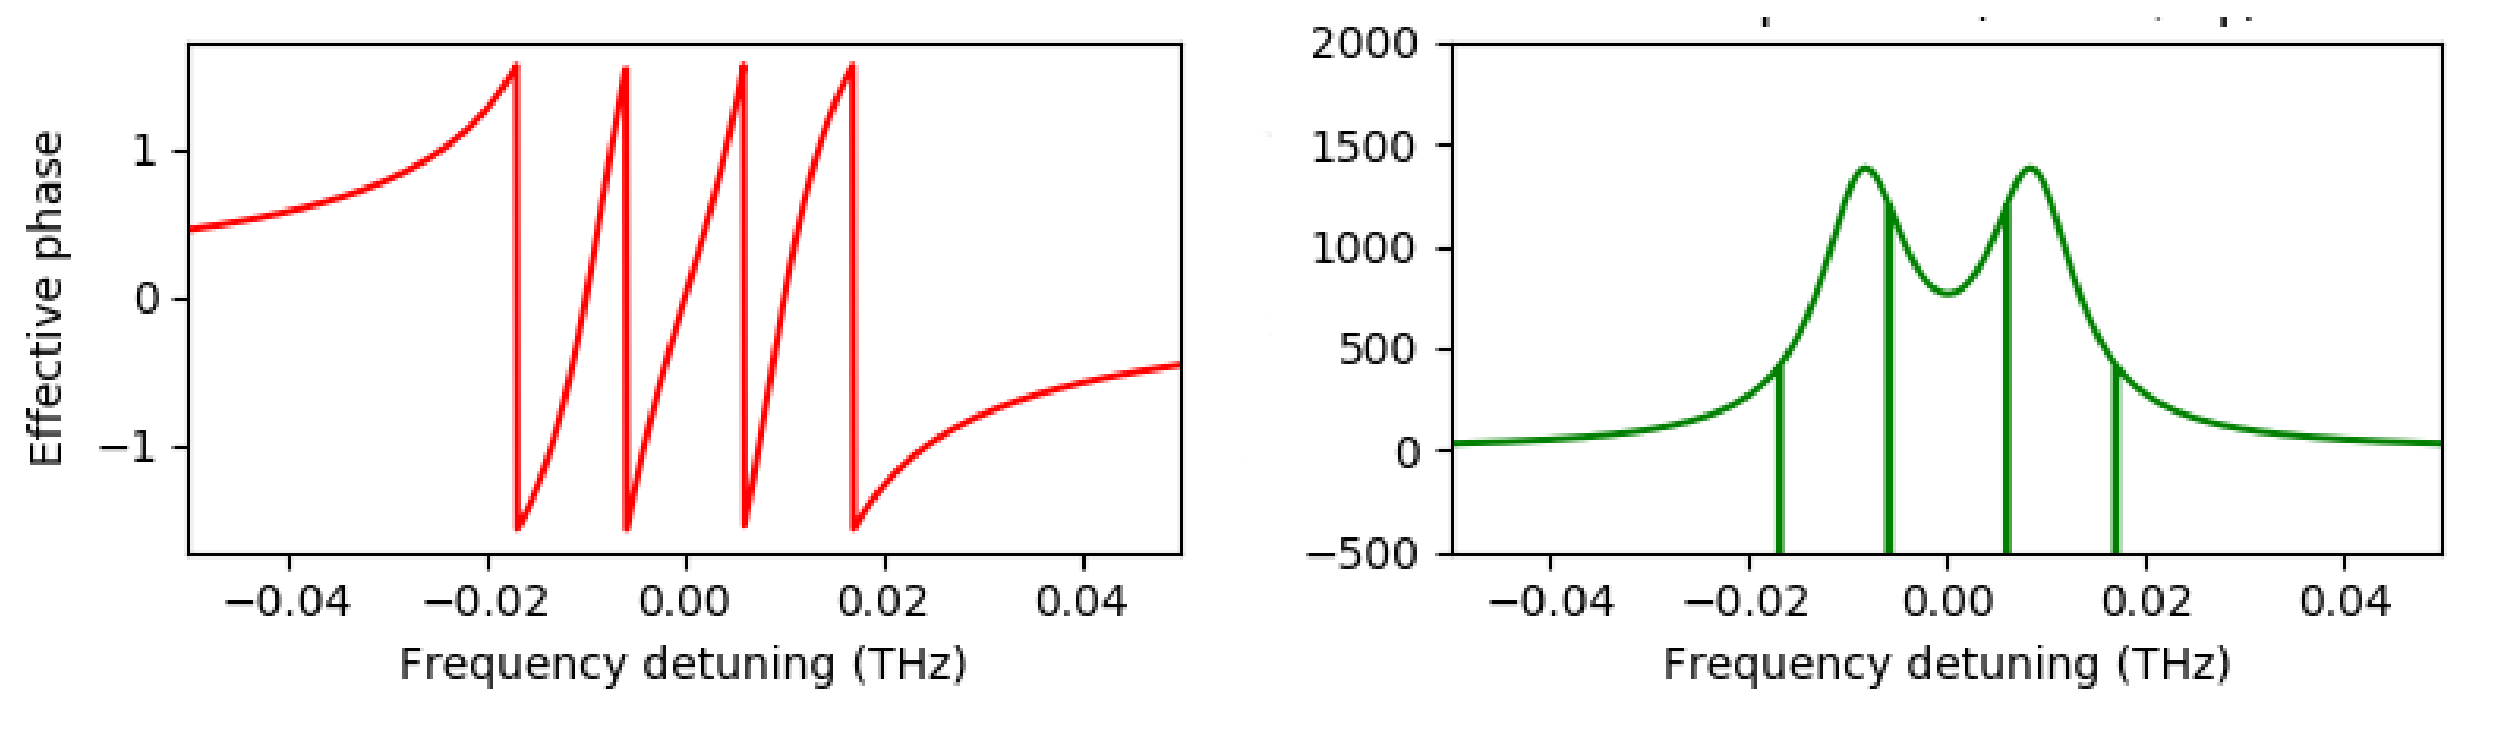
\includegraphics[scale=0.35]{EIT_gain12_phase.eps}
\caption{Phase and Group index of a resonator system with gain in both resonators.}
\end{figure}

When the gain coefficient $g$ becomes greater than $\alpha$, then the whole transmission graph flips about the x-axis and we now see a distinct spectrum with an reversed EIT shown in figure 3.11.

\begin{figure}[h]
\centering
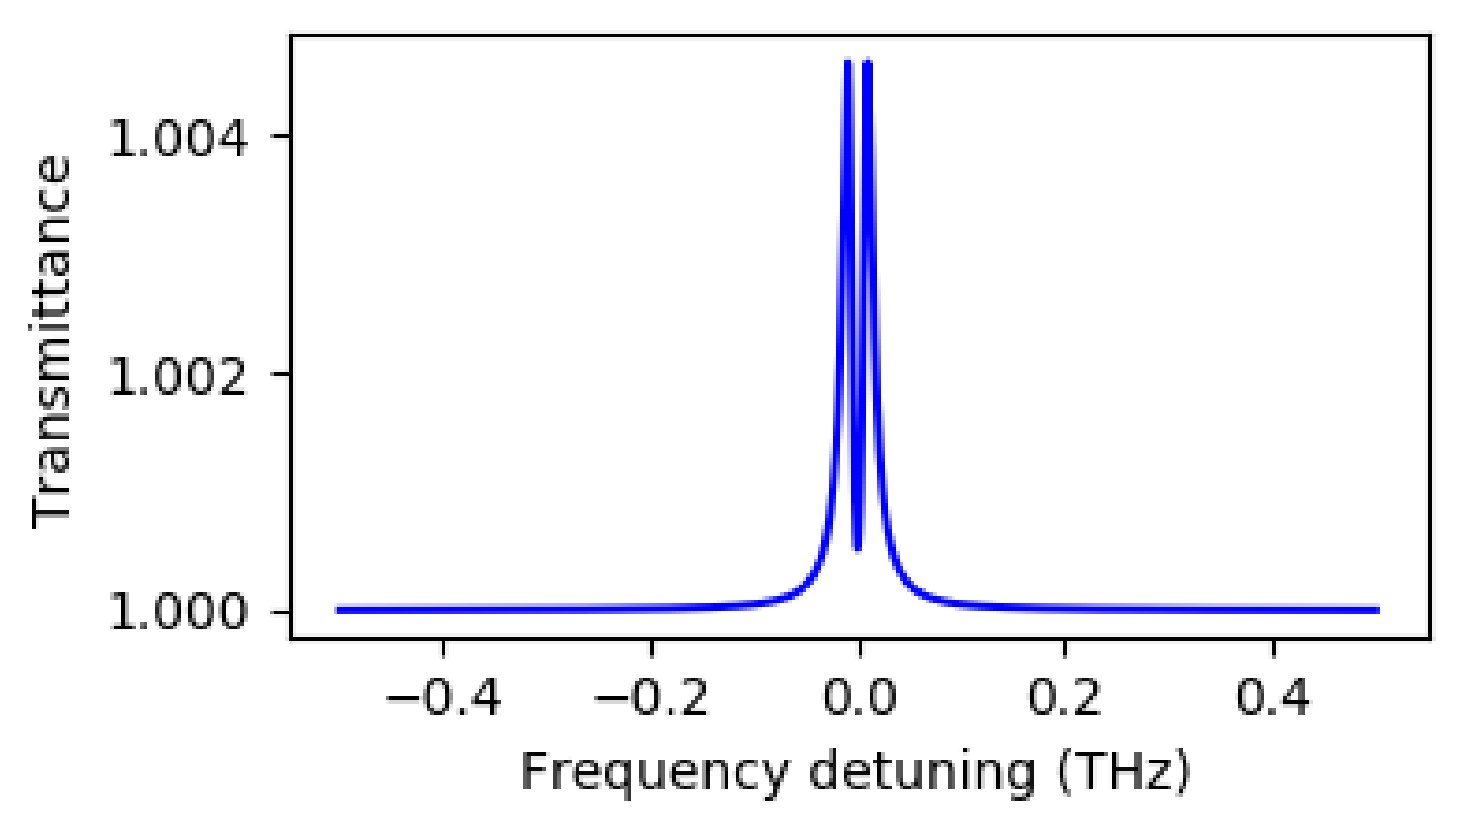
\includegraphics[scale=0.35]{EIT_gain12b.eps}
\caption{Flipping of the EIT spectrum when gain coefficient is bigger than the attenuation coefficient.}
\end{figure}

This flipping of the transmission does not affect the dispersion of the medium which means the effective phase and the group index of the system remains the same in this case as well. However, we now have a transmission peak which is above the 1 mark on the graph meaning we have compensated for all the losses in the system and also we have generated extra light.

\newpage


\section{Electromagnetically Induced Absorption}
A similar phenomenon in which quantum interferences causes a narrow dip in the transmission spectrum of the system is known as Electromagnetically Induced Transparency (EIA). EIA is believed to occur when the probability amplitudes of the exciting electrons from a three level system, one coming from the groud state due to the probe laser and the other coming from the metastable state due to control laser of high intensity, interferes constructively thus enhancing the absorption in the resonants frequencies and no light is transmitted in that narrow bandwidth of the spectrum.
As a whole, EIA is not a very well understood phenomenon and its classical explaination lacks the true esscence.

\section{Coupled Resonator Induced Absorption} 
 
Coupled resonator system as discussed above also displays electromagnetically induced absorption. The optical analogue of EIA is known as CRIA. CRIA can give us both fast light and slow light, most of the light in the resonant bandwidth is absorbed thus its applications are limited. 

\begin{figure}[h]
\centering
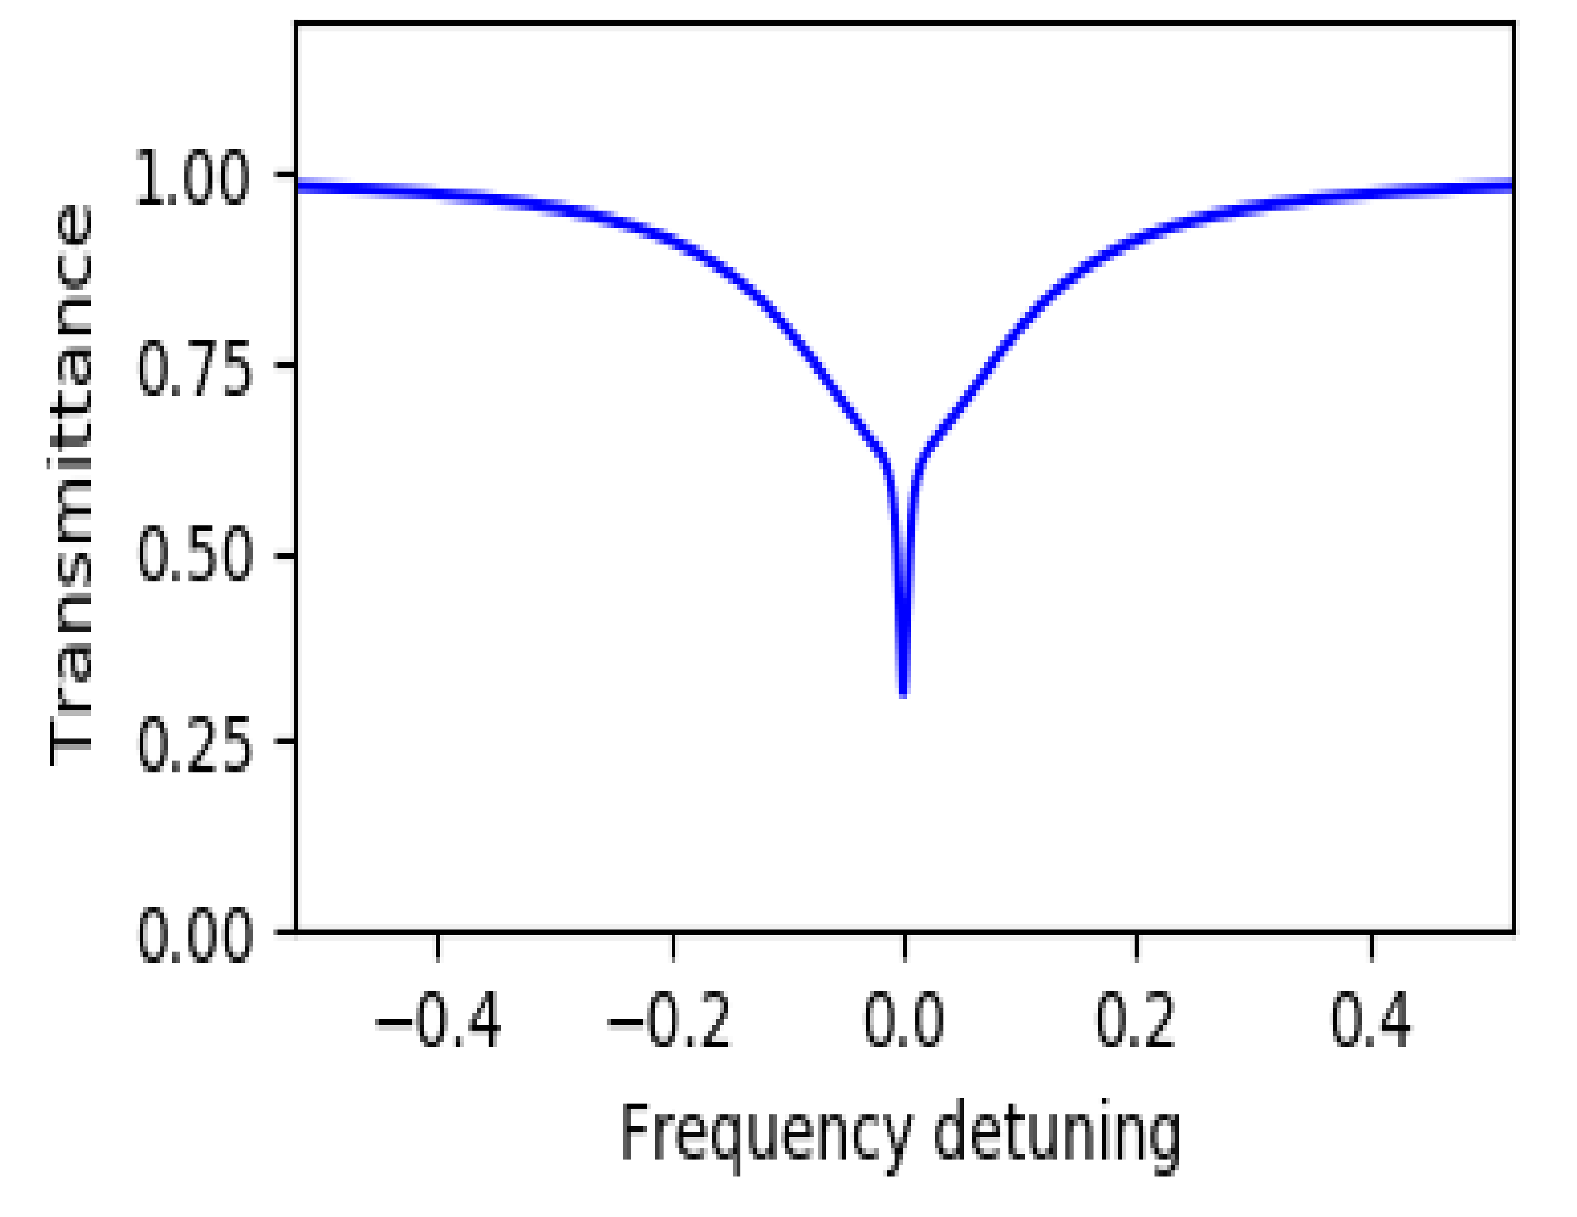
\includegraphics[scale=1]{EIA_basic.eps}
\caption{Coupled Resonator Induced Absorption in a coupled resonator system.}
\end{figure}
  

\section{CRIA with gain}
Now we will observe the behavior of the transmission spectrum of CRIA when we goin to introduce gain in it. Similarly, first we are going to activate gain in resonator 2, then into the resonator 1 and in last we activate and increase gain in both resonators simultaneously. 

\subsection{CRIA with slow light}
We wil first see the response of the CRIA (fig. 3.14) in active medium with having normal dispersion. shown in fig. 15, with its group index.

\begin{figure}[h]
\centering
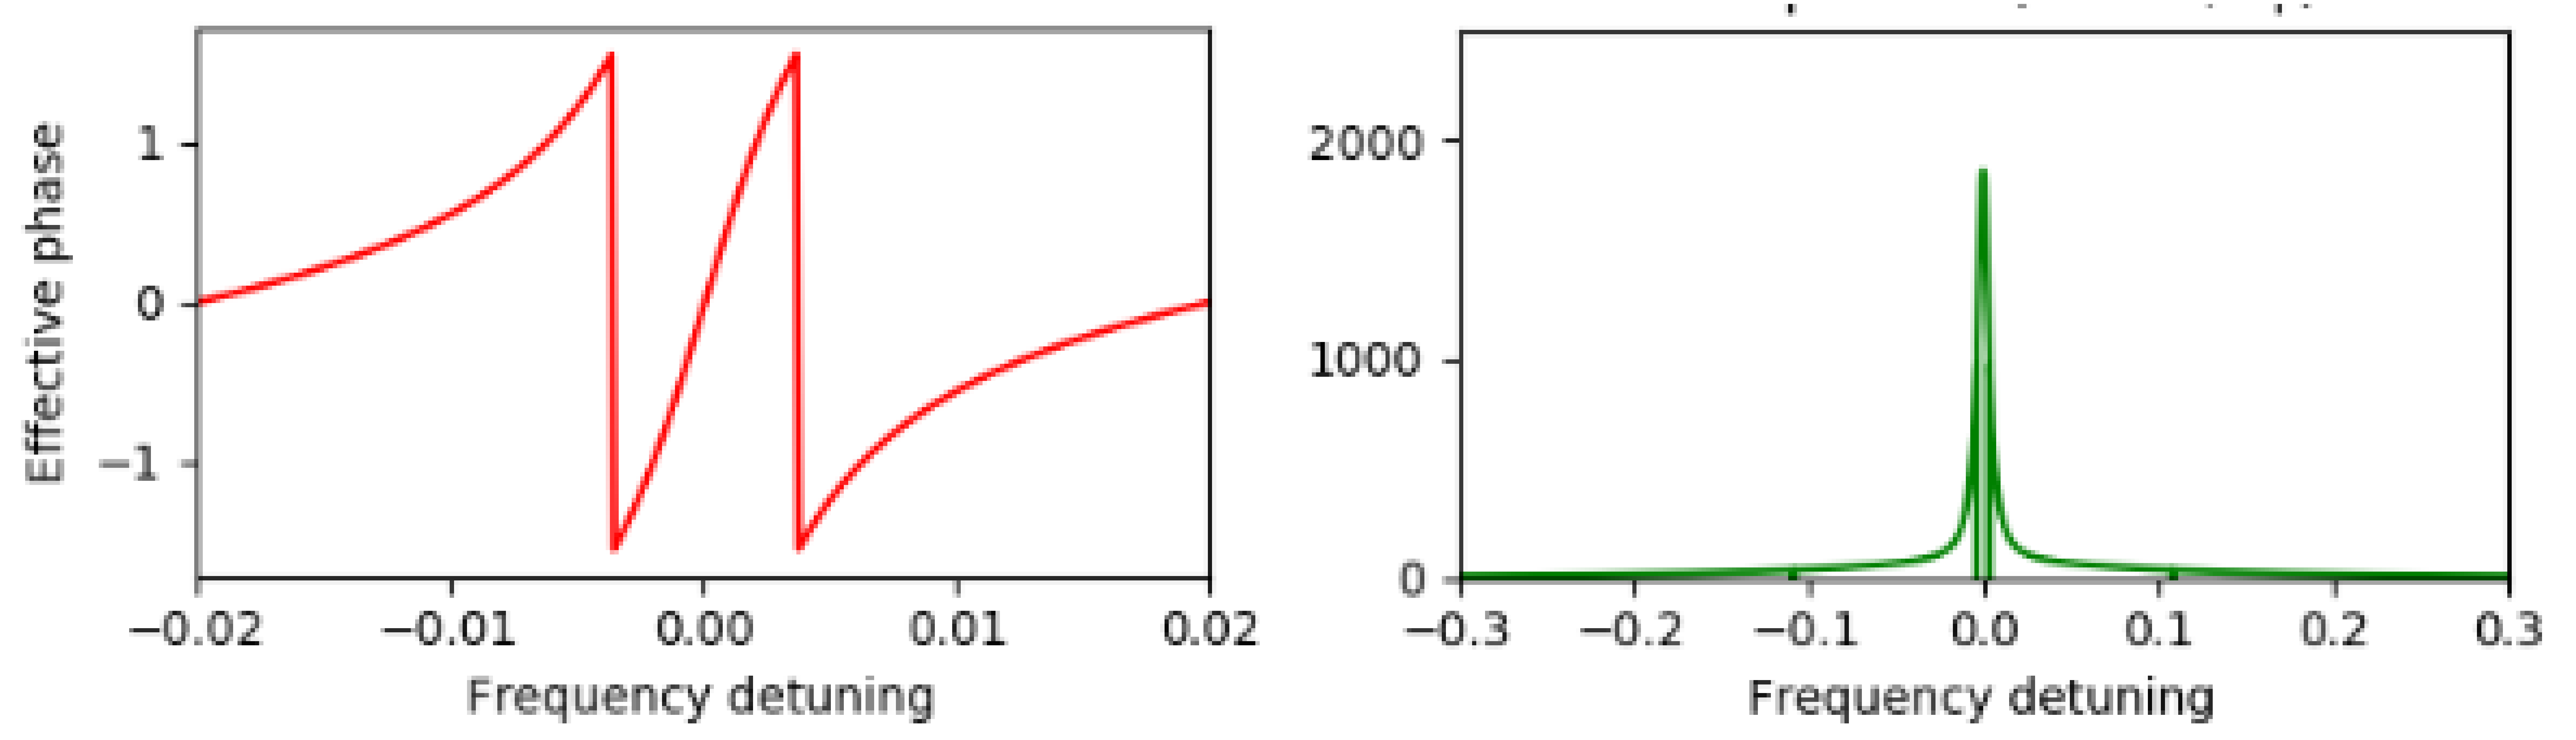
\includegraphics[width=1\textwidth]{EIA_gain_phase1.eps}
\caption{Phase and group index of CRIA.}
\end{figure}
  
\subsubsection{Introducing gain in resonator 2}
Now we activate gain in the second resonator such that $g \leqslant \alpha$ .  When the gain is closer to the value of $\alpha$ ( $g \to \alpha$) makes the EIA change into EIT type transmission.

\begin{figure}[h]
\centering
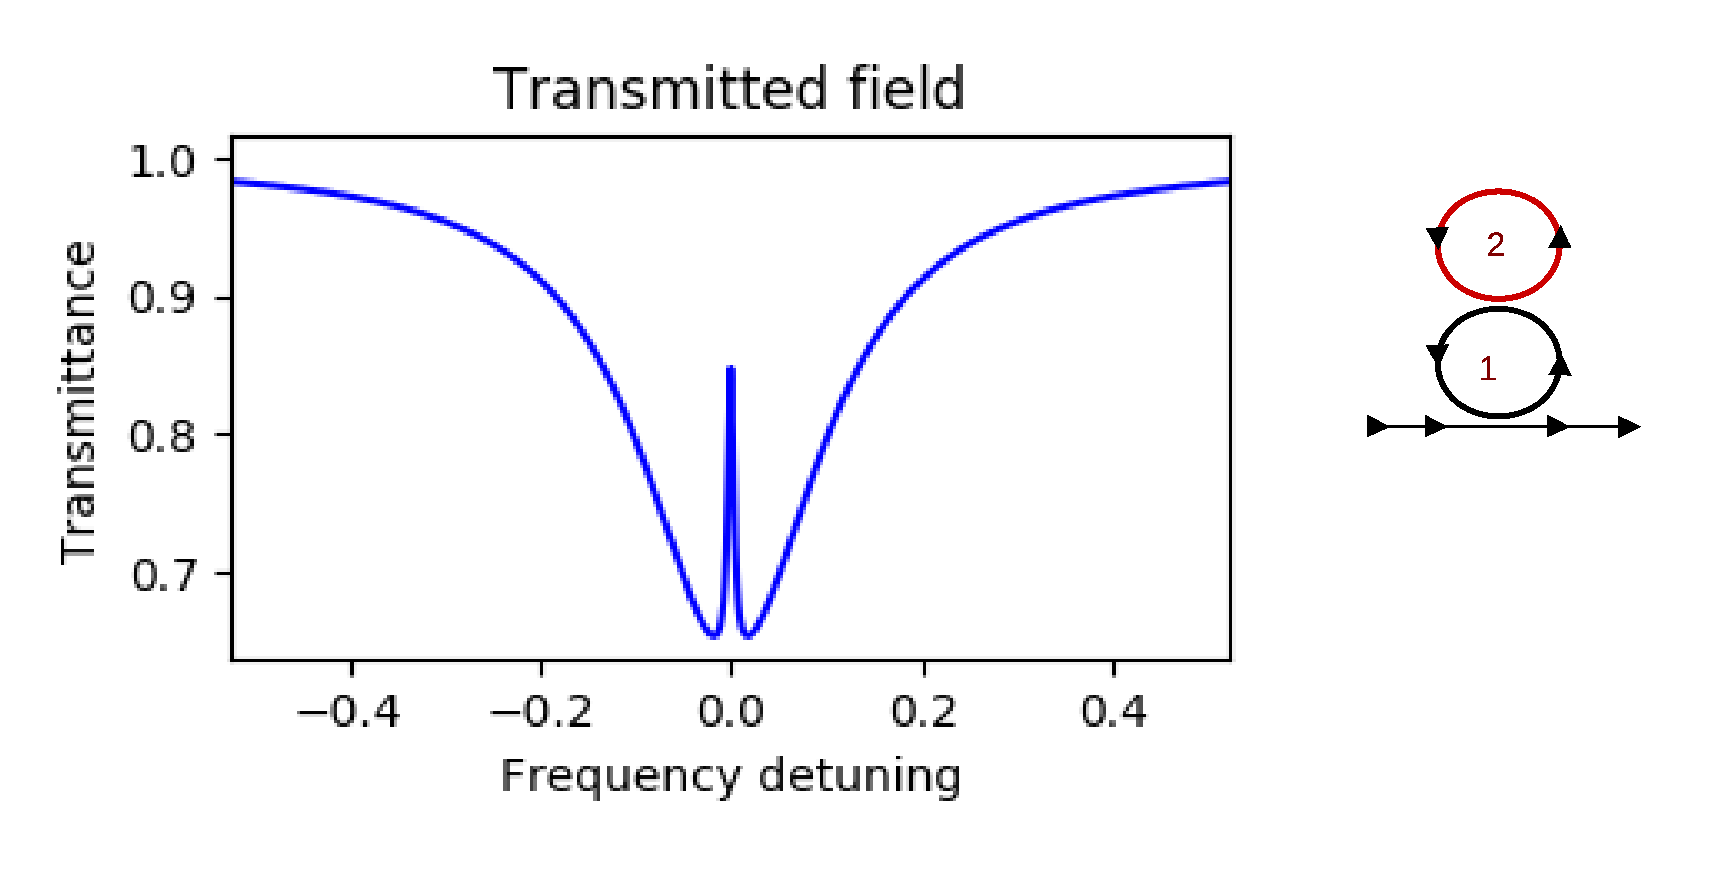
\includegraphics[scale=0.35]{EIA_to_EIT.eps}
\caption{EIA dip changes into an EIT type transmission.}
\end{figure}

The effective phase of the transmission changes from normal dispersion to anamolous dispersion. The group index displays negative value of $n_{g} \approx -4505$, meaning negative group delay and superluminal light.

\begin{figure}[h]
\centering
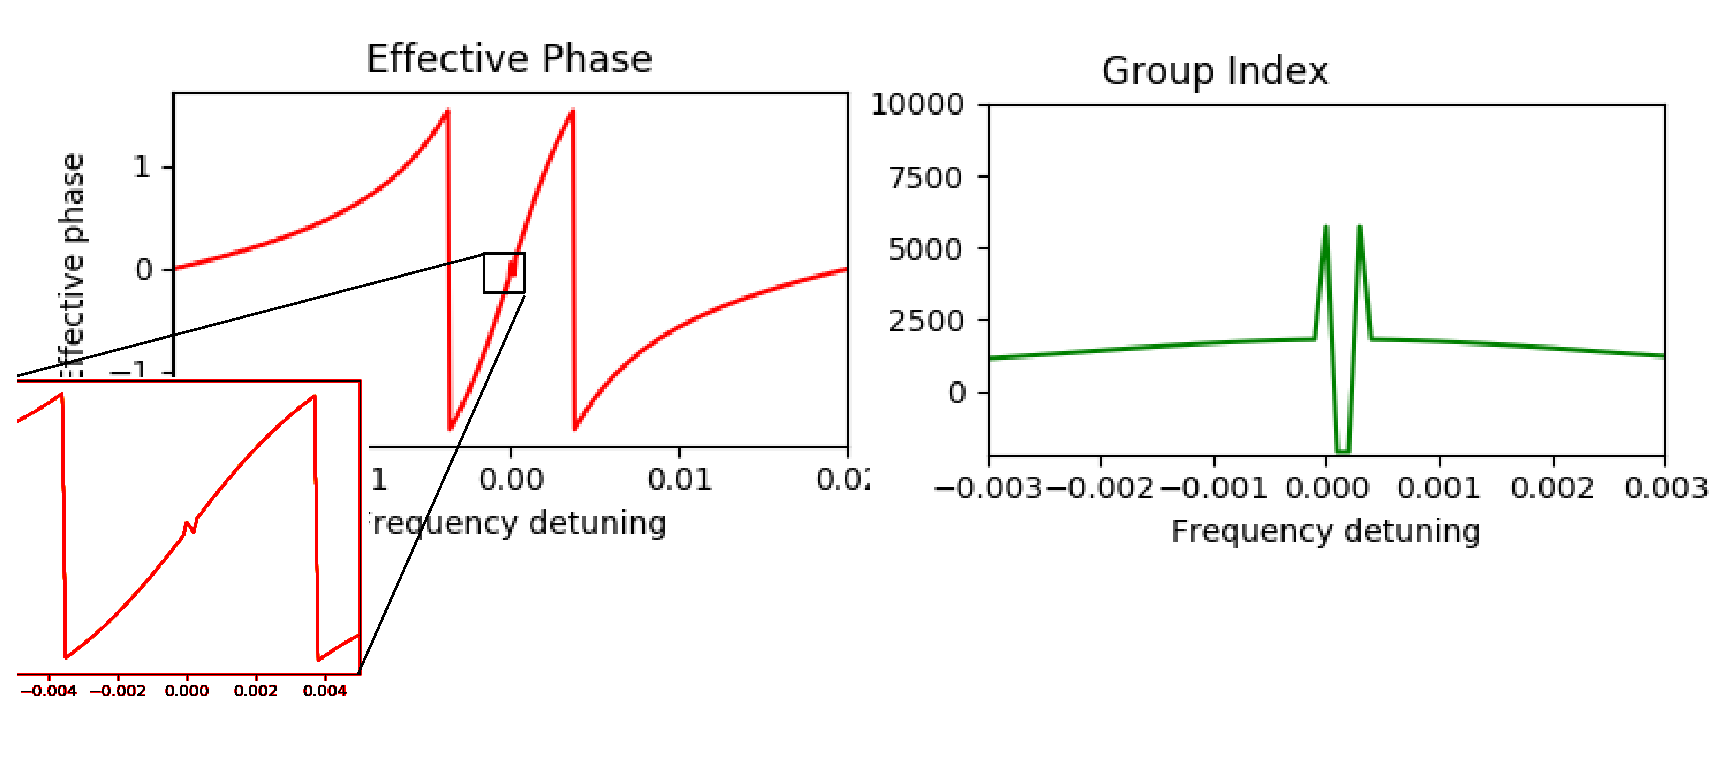
\includegraphics[scale=0.45]{EIA_to_EIT_phase.eps}
\caption{Phase of the system shown in red and group index in green.}
\end{figure}

\subsubsection{Introducing gain in resonator 1}
Now we activate gain in the first resonator shown in red and we see that the EIA resonance narrows down and becomes a sharp transmission dip.

\begin{figure}[h]
\centering
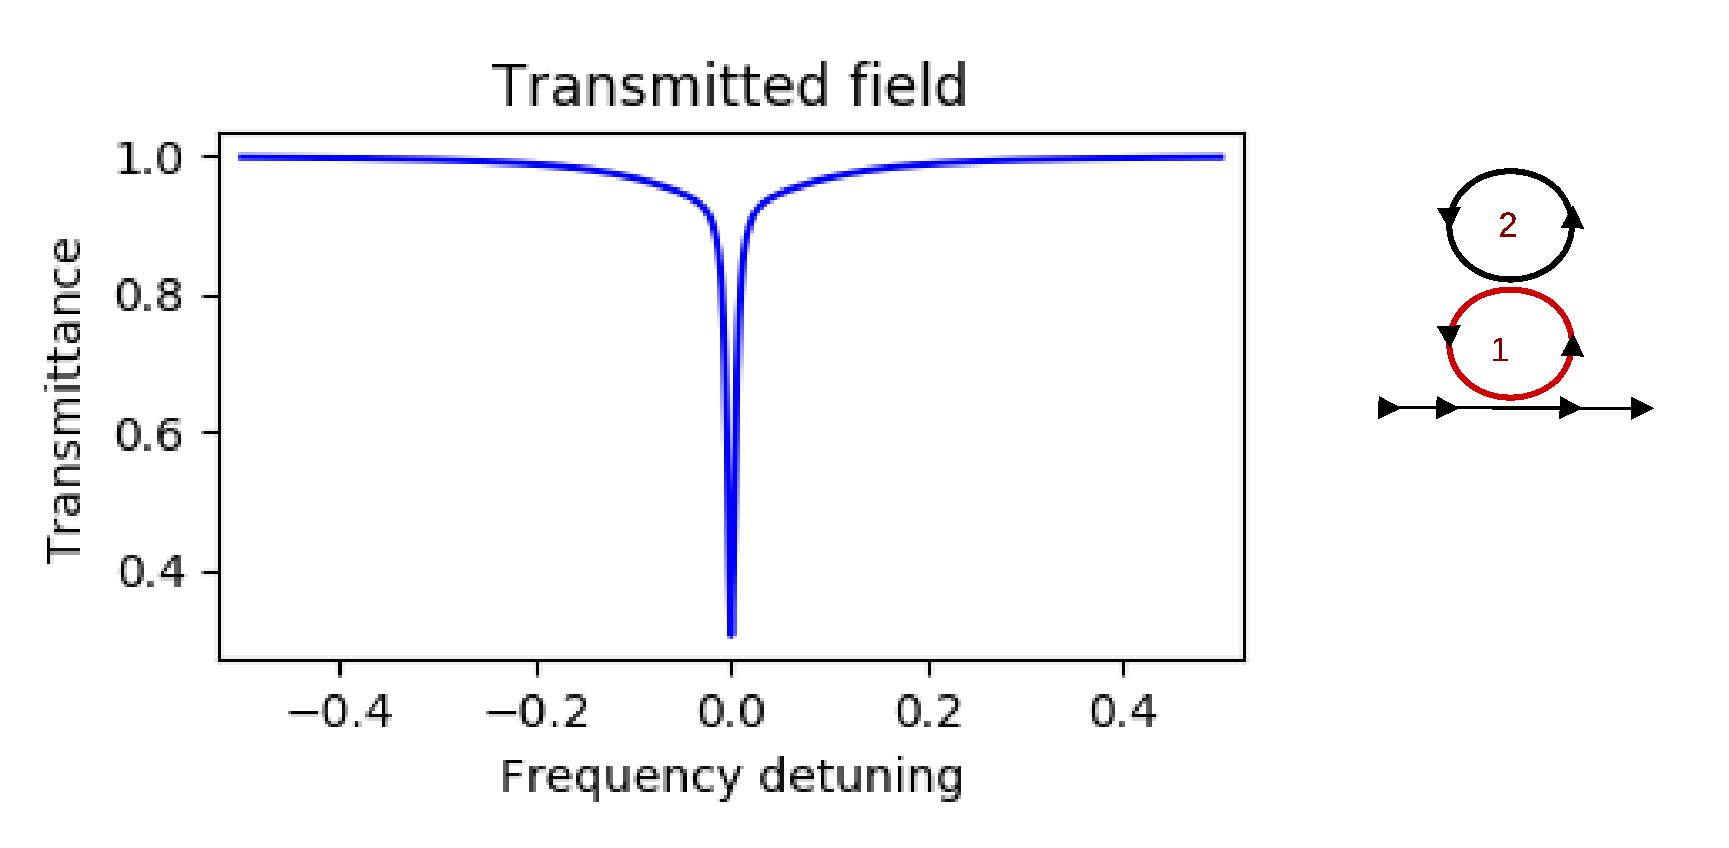
\includegraphics[scale=0.45]{EIA_gain1.eps}
\caption{CRIA with gain activated in resonator 1.}
\end{figure}

Phase and group index gives us slow light and normal dispersion.

\begin{figure}[h]
\centering
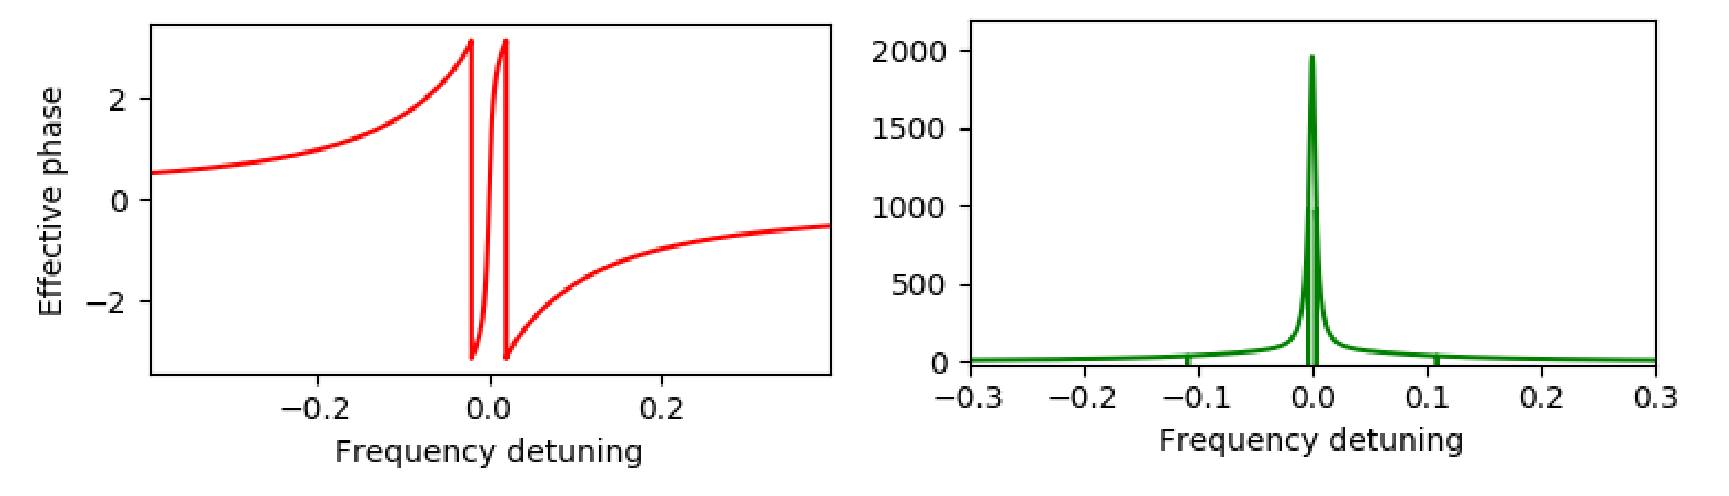
\includegraphics[scale=0.45]{EIA_gain1_phase.eps}
\caption{CRIA phase and group index.}
\end{figure}


\subsubsection{Introducing gain in both resonators}
Now we will activate gain in both of the resonators simultanously. We see no clear difference in the transmission spectrum when $g_{1} and g_{2} < \alpha$.

\begin{figure}[h]
\centering
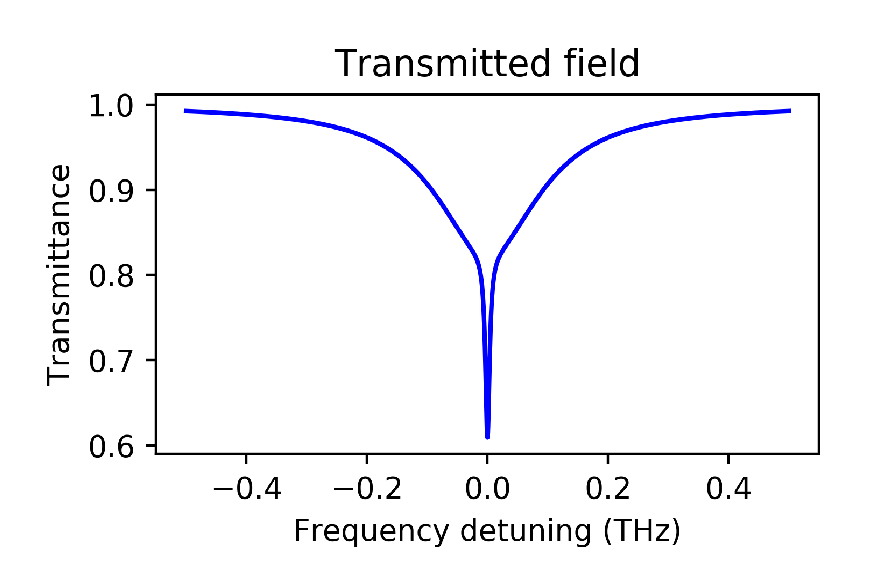
\includegraphics[scale=0.5]{EIA_gain12.eps}
\caption{CRIA with gain in both resonators.}
\end{figure}

The phase and group index is also shown

\begin{figure}[h]
\centering
\includegraphics[scale=0.5]{EIA_gain12_phase.eps}
\caption{CRIA phase in red and group index in green.}
\end{figure}

Again when $g \to \alpha$, the transmission spectrum values are very near to 1 now and we see anamolous dispersion in the effective phase of the system and negative group index of about $-4550$.

\begin{figure}[h]
\centering
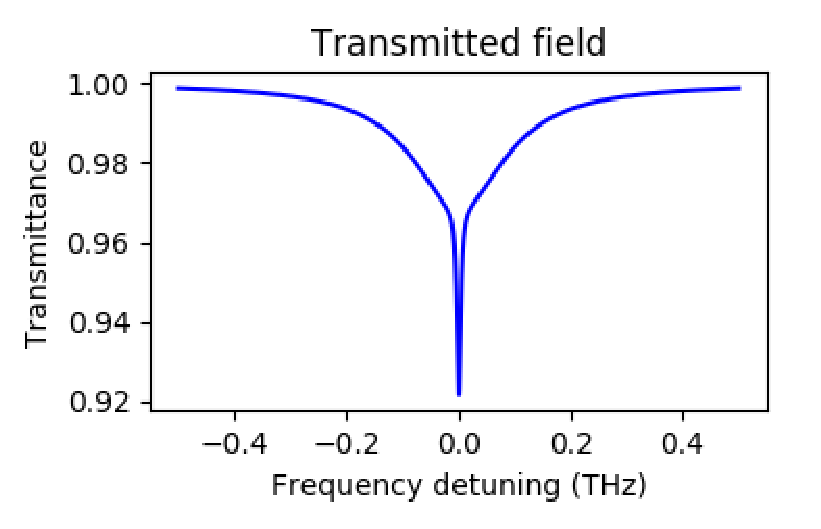
\includegraphics[scale=0.5]{EIA_gain12b.eps}
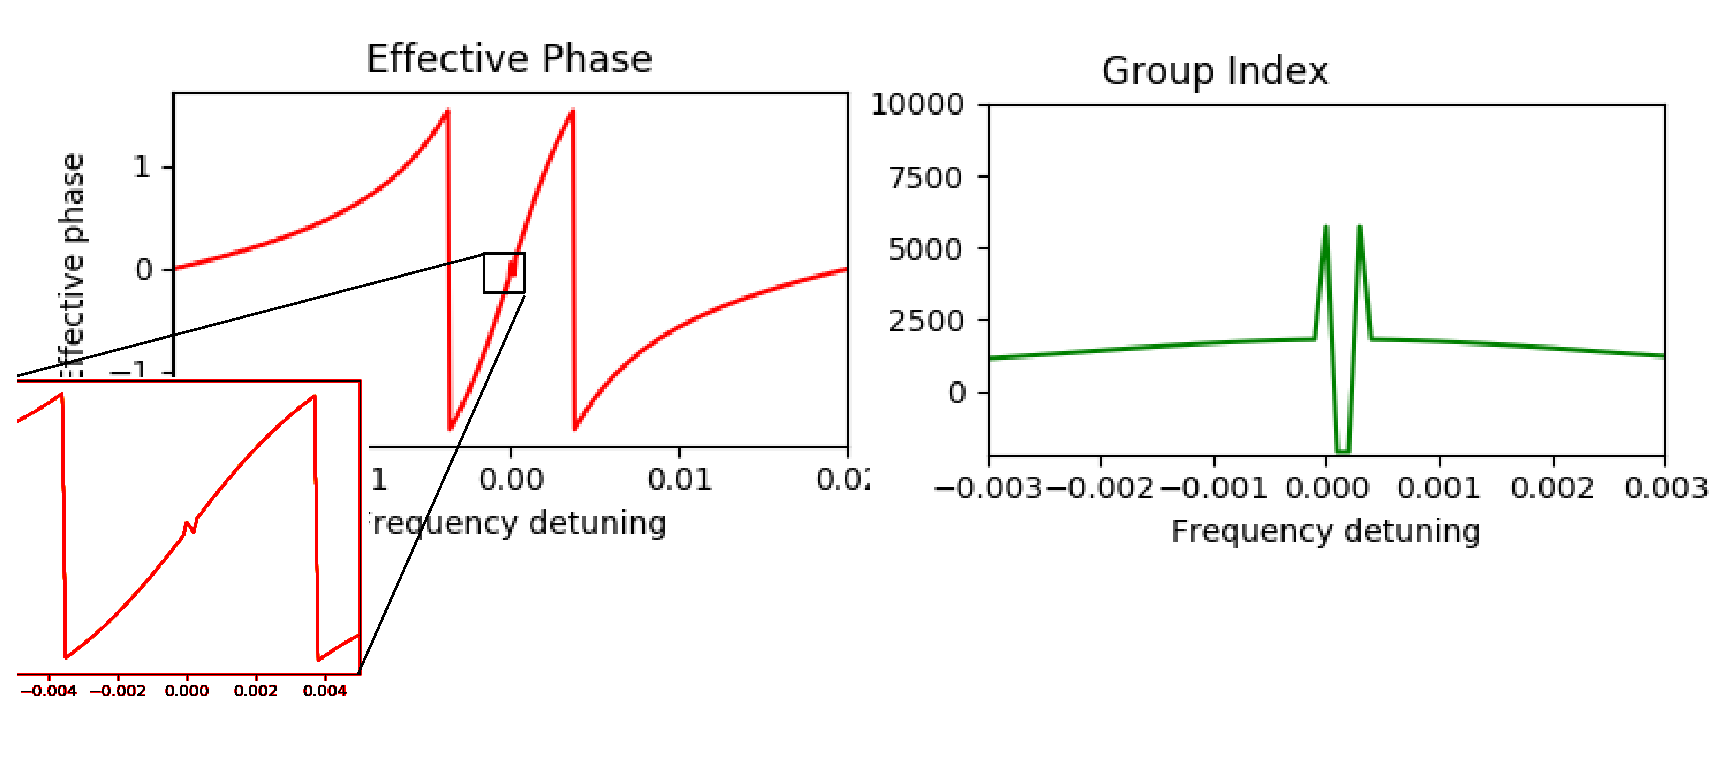
\includegraphics[scale=0.45]{EIA_to_EIT_phase.eps}
\caption{Phase of the system shown in red and group index in green.}
\end{figure}

Further increasing the gain we observe the spectrum flips over the horizontal axis and we see that our EIA has now become an EIT like transmission. The dispersion remains anamolous uptil few values of $g > \alpha$, but after significant introduction of gain in the system, we again see a transition from fast light to slow light and normal dispersion.

\begin{figure}[h]
\centering
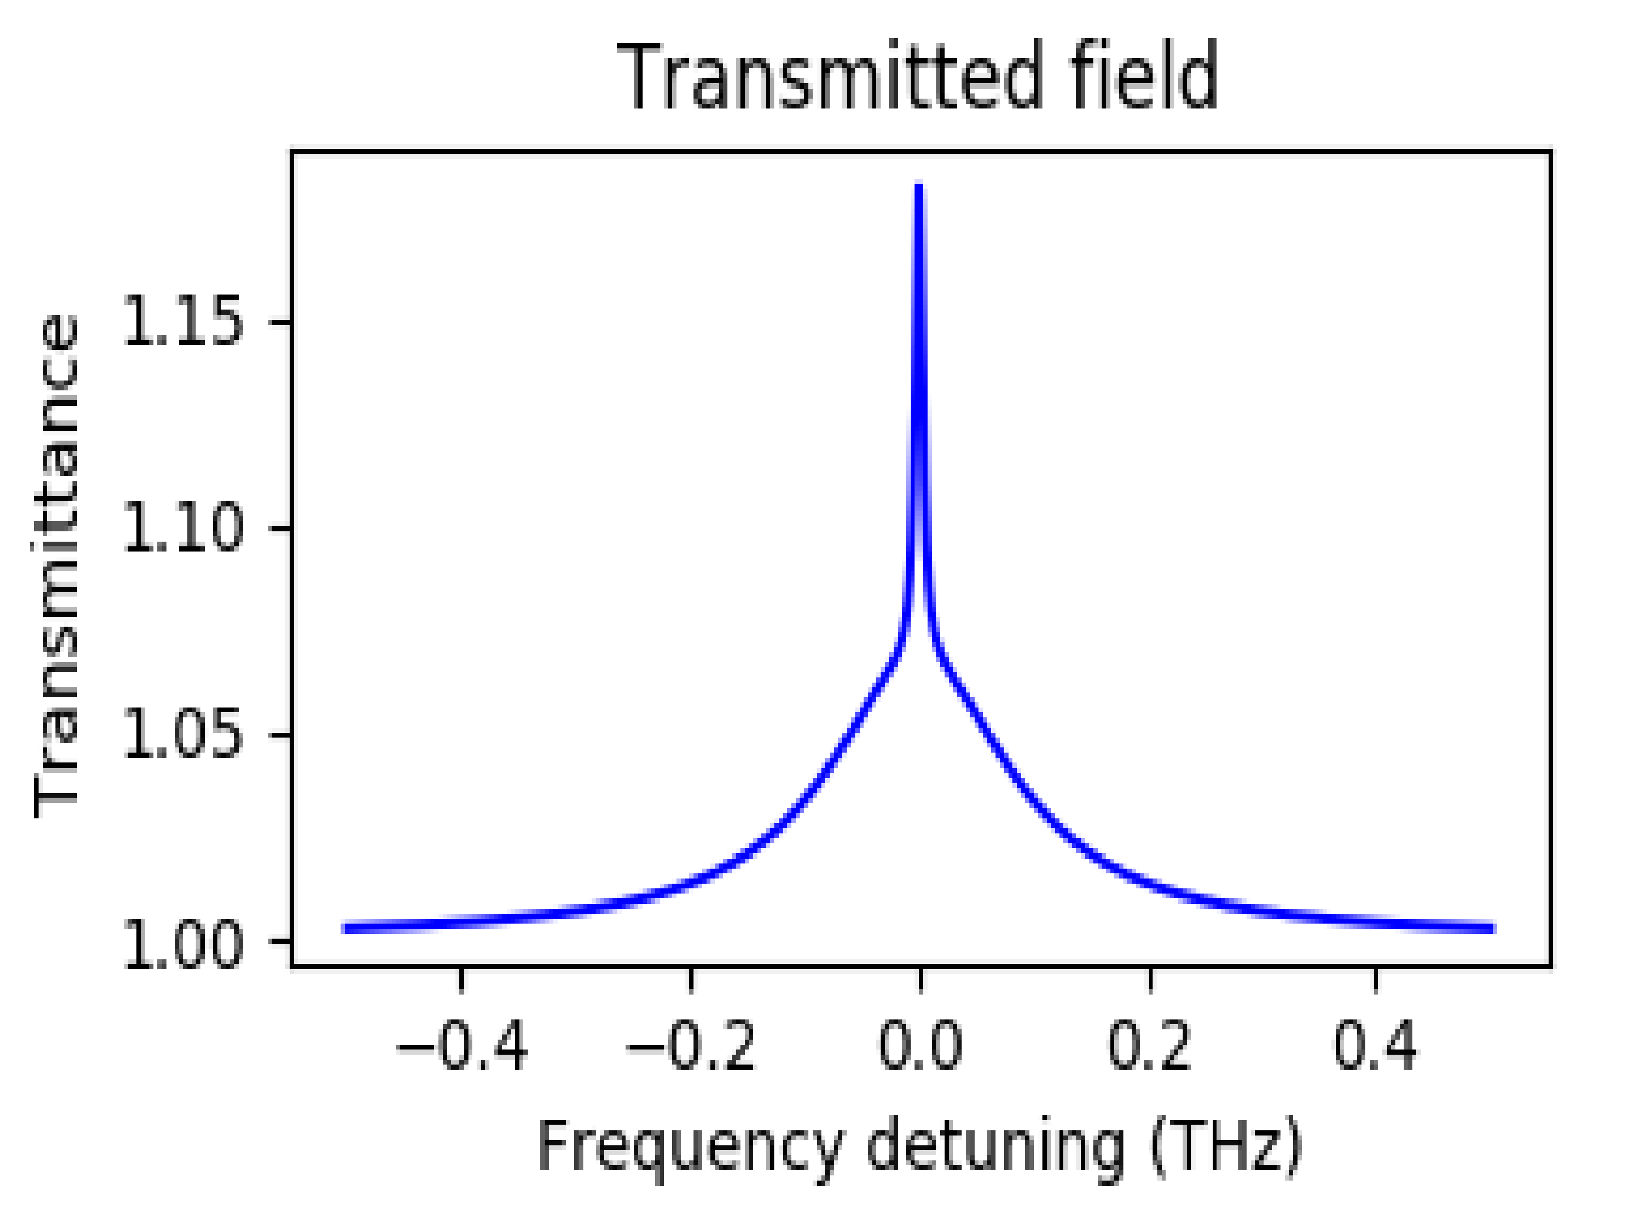
\includegraphics[scale=0.65]{EIA_gain12ab.eps}
\caption{Transmission of the system}
\end{figure}
\newpage
\begin{figure}[h]
\centering
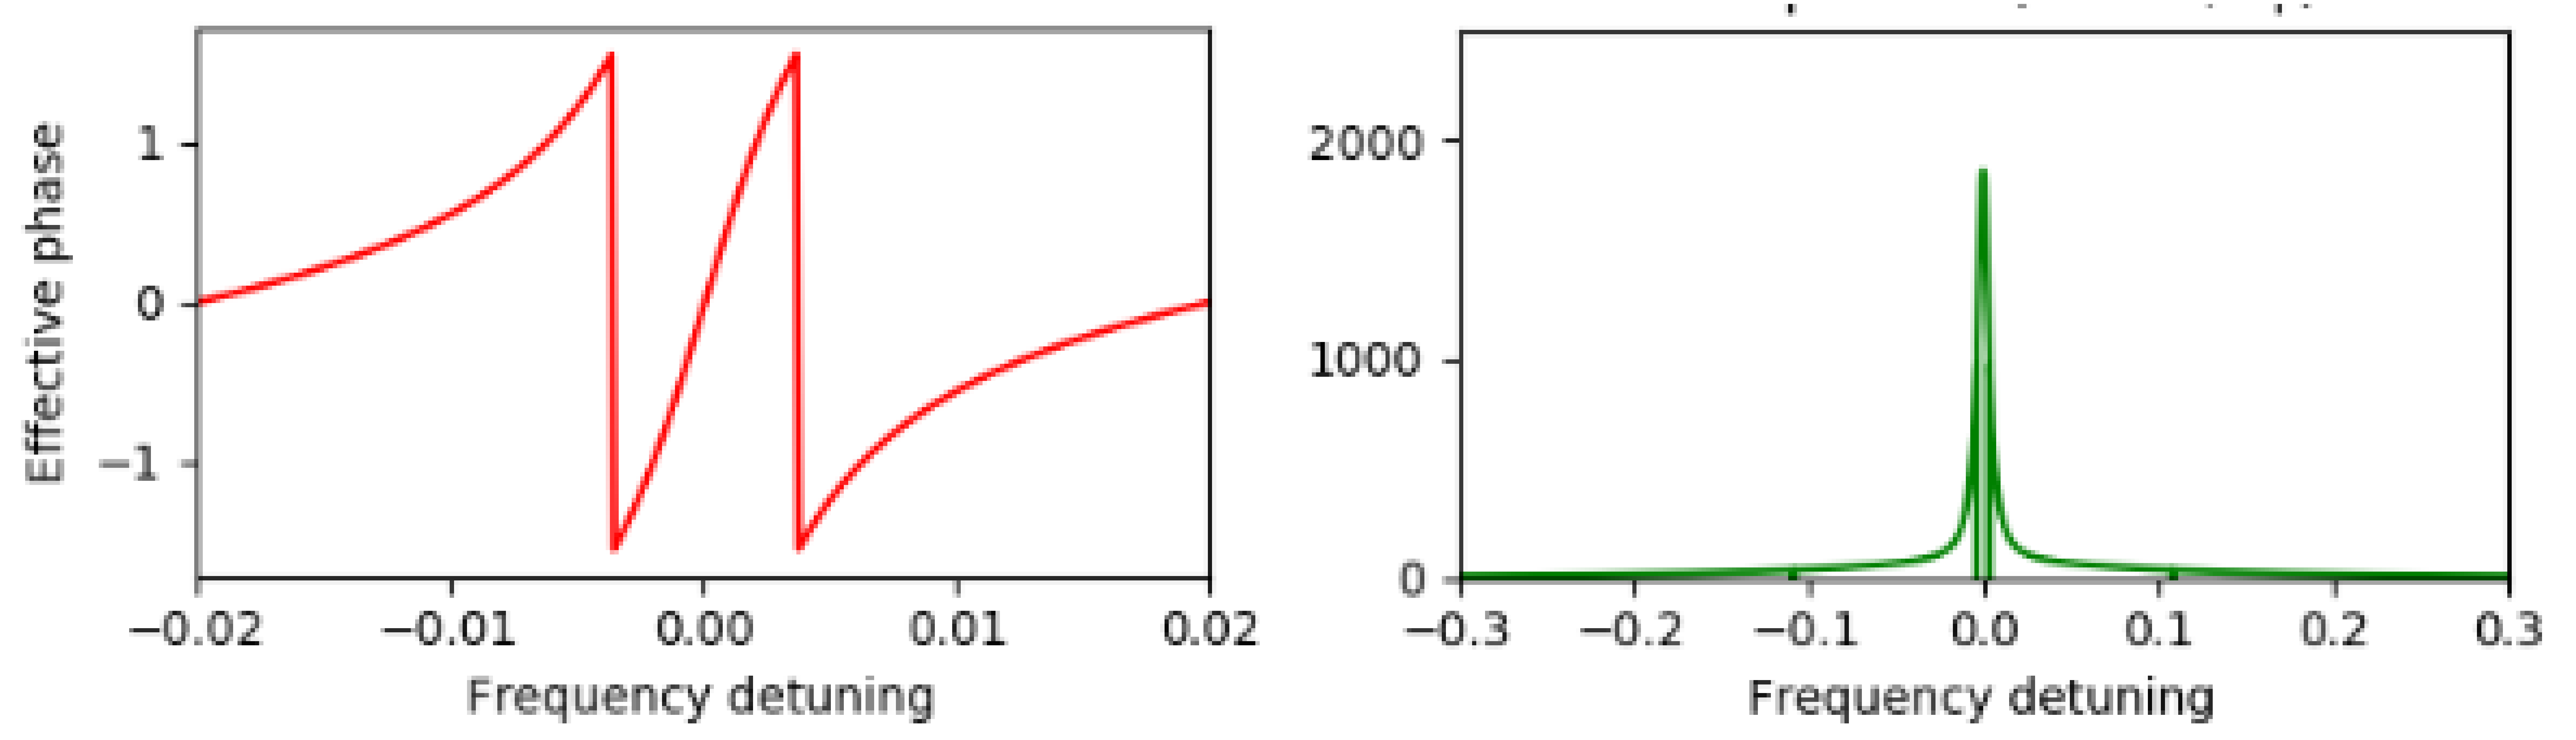
\includegraphics[width=1\textwidth]{EIA_gain_phase1.eps}
\caption{Phase and group index of the system.}
\end{figure}

\subsection{CRIA with fast light}
Now we will study CRIA which shows fast light with a passive resonator system and study the behavior when gain is introduced into it simultanously.

\begin{figure}[h]
\centering
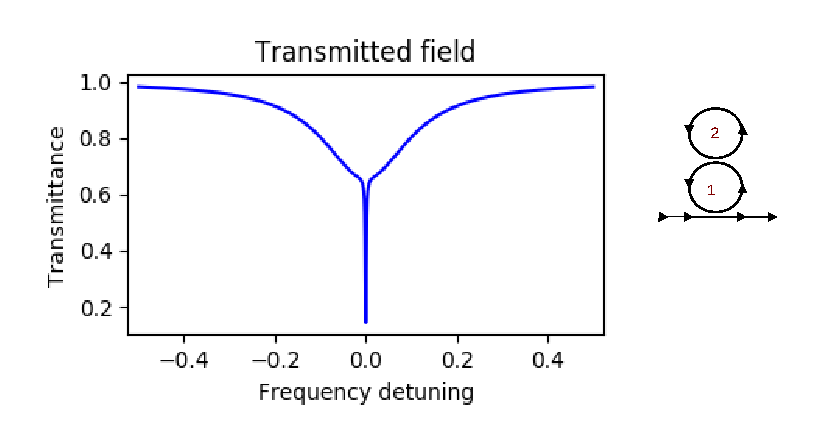
\includegraphics[scale=0.65]{EIAf_passive.eps}
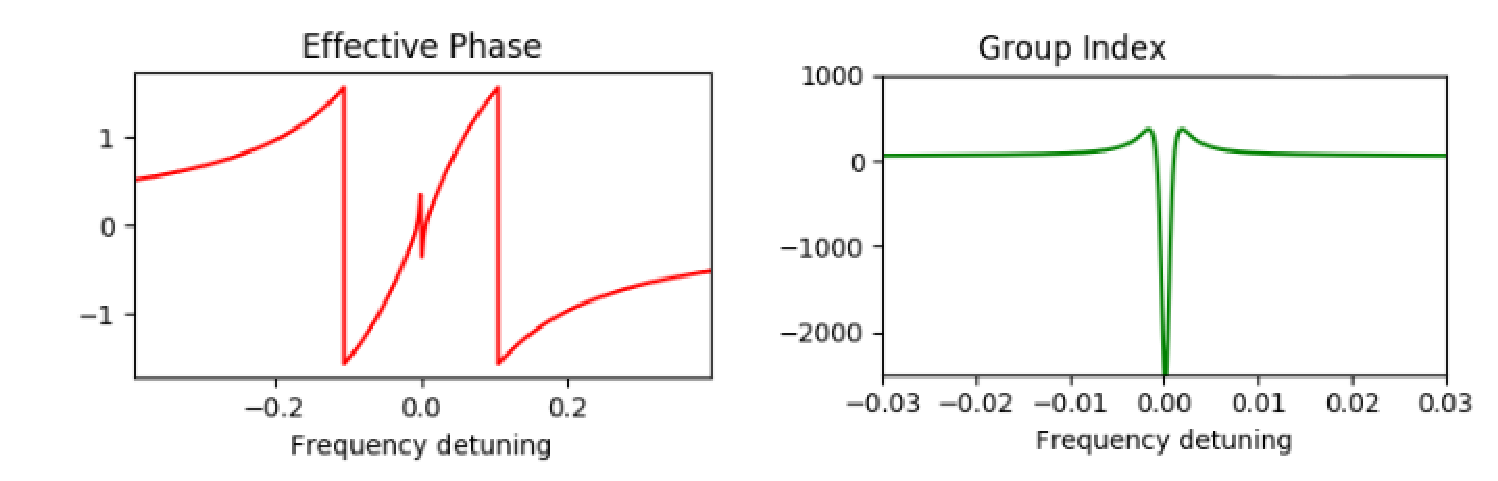
\includegraphics[scale=0.5]{EIAf_passive_phase.eps}
\caption{CRIA observed in a passive two resonator system.}
\end{figure}

\subsubsection{Introducing gain in resonator 2}
Now we activate gain in the second resonator shown in red and we see that the EIA resonance narrows down and becomes a sharp. Also the dispersion of the system changes as $g \approx \alpha$ and we see normal dispersion and a positive group index.

\begin{figure}[h]
\centering
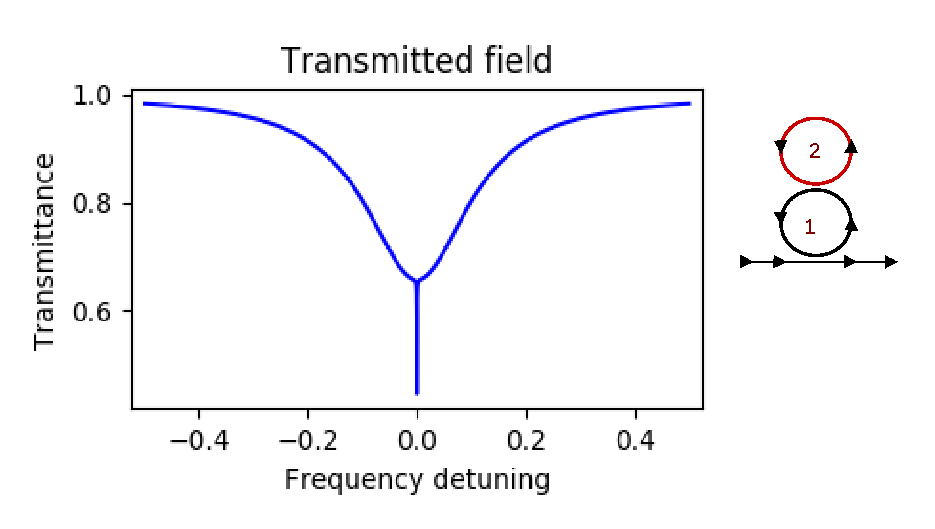
\includegraphics[scale=0.65]{EIAf_gain2.eps}
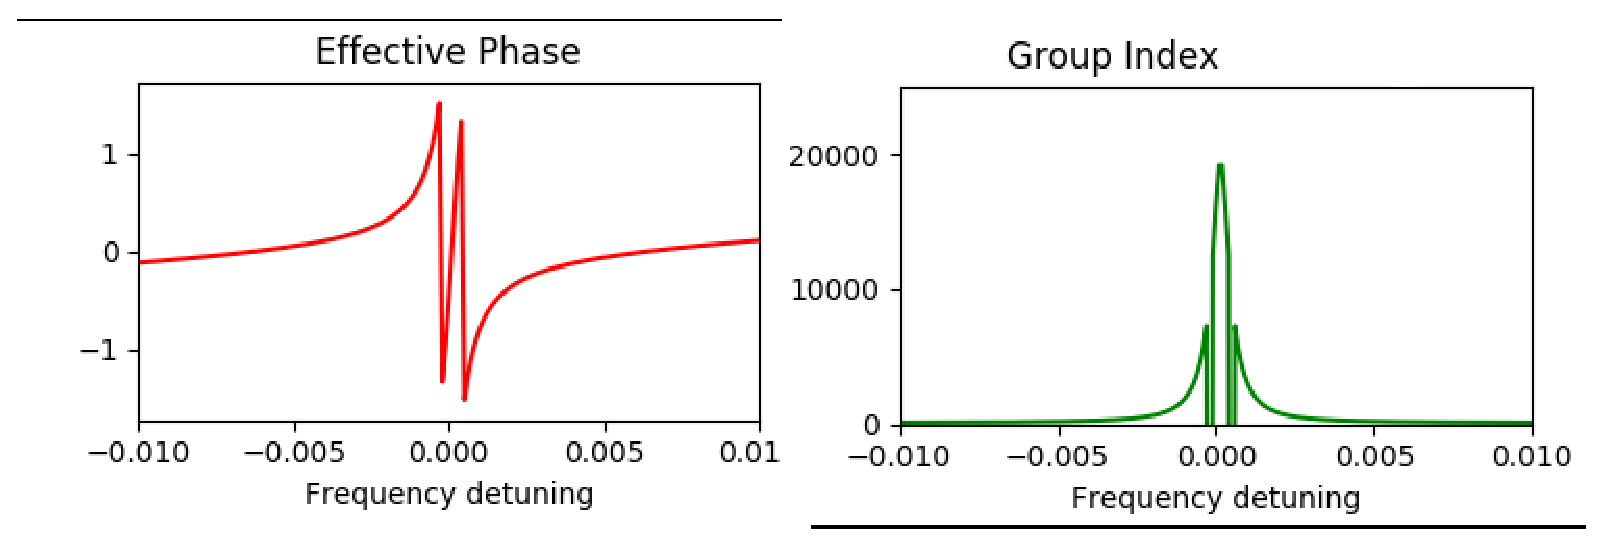
\includegraphics[scale=0.5]{EIAf_gain2_phase.eps}
\caption{Transition from fast to slow light in CRIA.}
\end{figure}

When gain of the system is higher than the losses, such that $g > \alpha$, then we see a change in transmission that the EIA dip has changed into an EIT peak with normal dispersion and positive group index.

\begin{figure}[h]
\centering
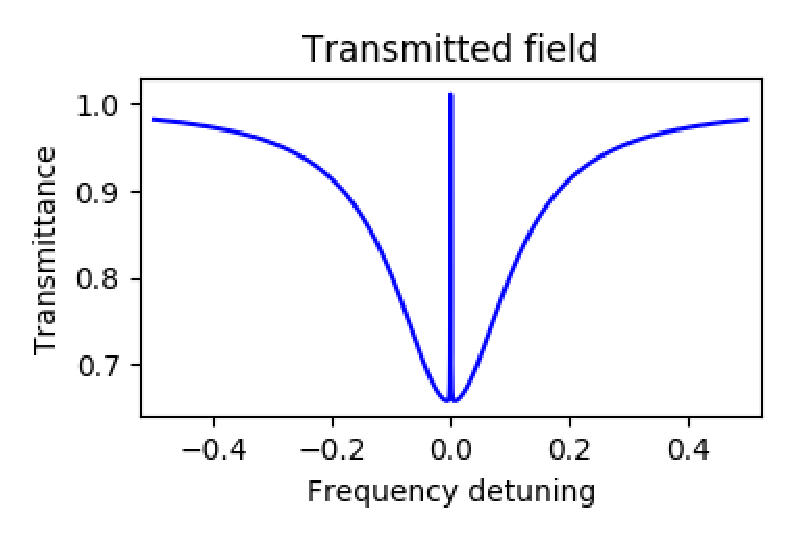
\includegraphics[scale=0.60]{EIAf_gain2a.eps}
\caption{Transmission dip transforming into an tranmission peak.}
\end{figure}

However, the effective phase and the group index remains the same even for this tranmission, but now we have more output light and less of our input signal is absorbed thus increasing its essence.
\newpage

\subsubsection{Introducing gain in resonator 1}
Now we activate gain in the first resonator. We see that the EIA resonance narrows down and becomes a sharp dip. Also we see two off resnonces starts to appear. As $g \approx \alpha$, the dip is narrow and touches the zero in the graph meaning almost all of the light is absorbed. We still see fast light and negative group index from here but most of the light is absorbed. The transmission spectrum is shown for $g > \alpha$.

\begin{figure}[h]
\centering
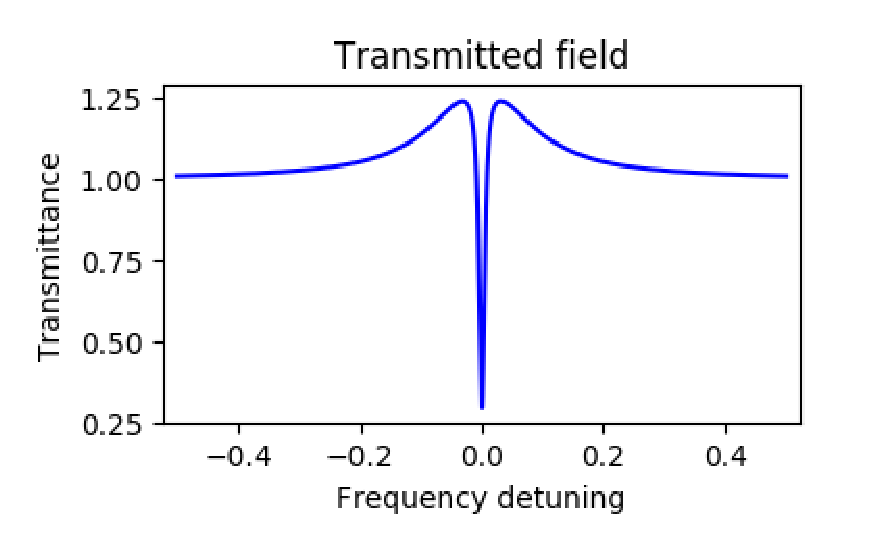
\includegraphics[scale=0.60]{EIAf_gain1.eps}
\caption{Transmission dip of CRIA with gain in resonator 1.}
\end{figure}

\subsubsection{Introducing gain in both resonator}
When we introduce gain in both of the resonator simultaneously, then we see similar effects as with gain activated in resonator 2. But the transmission dip changes into a peak when $g > \alpha$ meaning all the losses are compensated and we have normal dispersion with an high amount of transmission.

\begin{figure}[h]
\centering
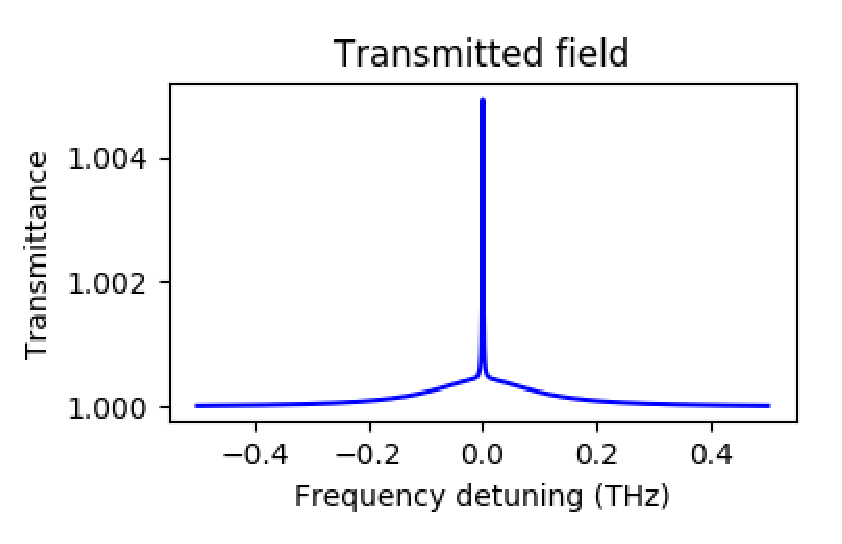
\includegraphics[scale=0.60]{EIAf_gain12.eps}
\caption{Transmission dip transforming into an tranmission peak.}
\end{figure}

\begin{figure}[h]
\centering
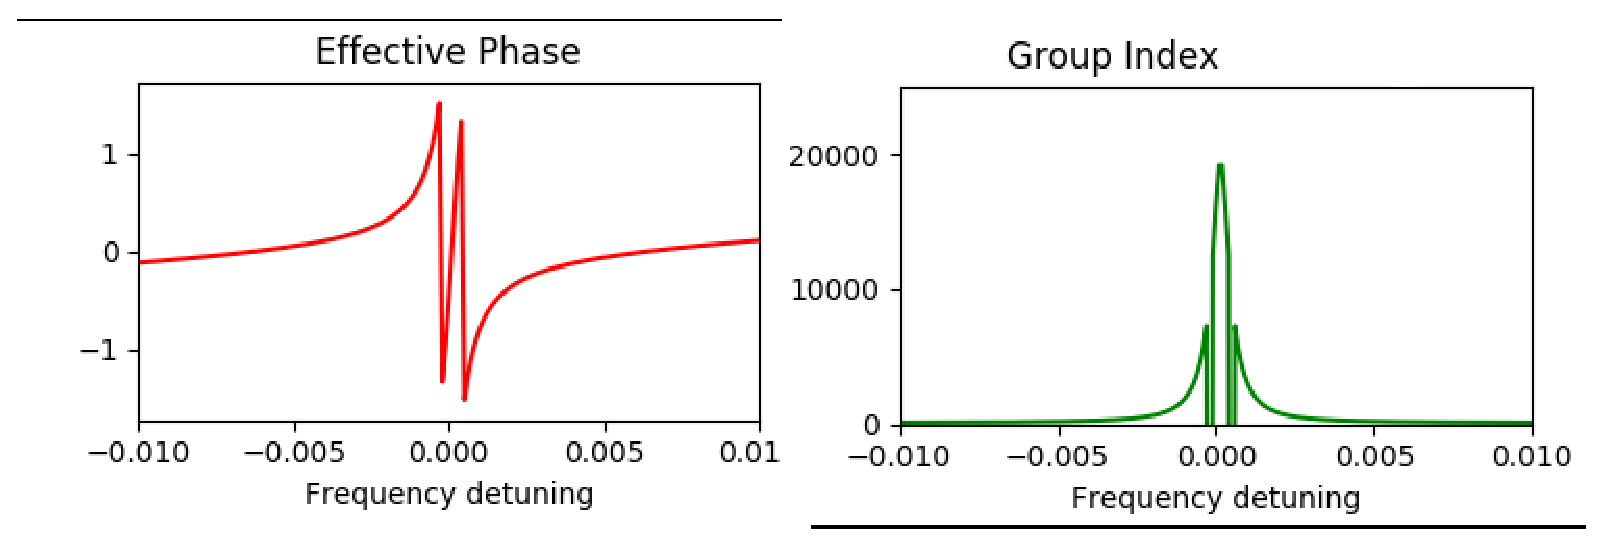
\includegraphics[scale=0.60]{EIAf_gain2_phase.eps}
\caption{Respective phase and group index of the system.}
\end{figure}


\section{Conclusion}
We have clearly observed by studying the properties of different cases of a coupled resonator system. This observation told us that when we introduce gain into the system, we can see drastic changes in the transmission and phase spectrum of the system thus affecting the group delay and dispersion of the system. This allowed acheive gain tunability in these system which means that we can tune between fast and slow light by simply introducing gain inside the system.

\newpage
\section*{References}
\addcontentsline{toc}{section}{References}

\paragraph{\normalfont \large $[1]$ Electromagnetically Induced Transparency, Stephen E. Harris, Physics Today, July 1997 \\ 
\\$[2]$ Coupled-resonator-induced transparency, PHYSICAL REVIEW A 69, 063804 (2004)
\\$[3]$ What is and what is not electromagnetically induced transparency in whispering-gallery microcavities, DOI:10.1038/ncomms6082, Published 24 Oct 2014 \\
\\$[4]$  Induced transparency and absorption in coupled whispering gallery microresonators, PHYSICAL REVIEW A 71, 043804, published 5 April 2005\\
\\$[5]$  }